\PassOptionsToPackage{unicode}{hyperref}
\documentclass[aspectratio=1610, 11pt]{beamer}

\usepackage{amsmath}
\usepackage{amssymb}
\usetheme{tudo}

\title{Datenstrukturen, Algorithmen und Programmierung~2}
\author[A.~Coja-Oghlan]{Amin Coja-Oghlan}
\institute[DAP2]{Lehrstuhl Informatik 2\\Fakult\"at f\"ur Informatik}

\newcommand\dist{\mathrm{dist}}
\renewcommand{\vec}[1]{\boldsymbol{#1}}
\newcommand\NULL{{\tt NULL}}
\newcommand\dd{\mathrm d}
\newcommand\eul{\mathrm e}
\newcommand\cA{\mathcal A}
\newcommand\cB{\mathcal B}
\newcommand\cC{\mathcal C}
\newcommand\cD{\mathcal D}
\newcommand\cE{\mathcal E}
\newcommand\cF{\mathcal F}
\newcommand\cG{\mathcal G}
\newcommand\cH{\mathcal H}
\newcommand\cI{\mathcal I}
\newcommand\cJ{\mathcal J}
\newcommand\cK{\mathcal K}
\newcommand\cL{\mathcal L}
\newcommand\cM{\mathcal M}
\newcommand\cN{\mathcal N}
\newcommand\cO{\mathcal O}
\newcommand\cP{\mathcal P}
\newcommand\cQ{\mathcal Q}
\newcommand\cR{\mathcal R}
\newcommand\cS{\mathcal S}
\newcommand\cT{\mathcal T}
\newcommand\cU{\mathcal U}
\newcommand\cV{\mathcal V}
\newcommand\cW{\mathcal W}
\newcommand\cX{\mathcal X}
\newcommand\cY{\mathcal Y}
\newcommand\cZ{\mathcal Z}
\newcommand\fA{\mathfrak A}
\newcommand\fB{\mathfrak B}
\newcommand\fC{\mathfrak C}
\newcommand\fD{\mathfrak D}
\newcommand\fE{\mathfrak E}
\newcommand\fF{\mathfrak F}
\newcommand\fG{\mathfrak G}
\newcommand\fH{\mathfrak H}
\newcommand\fI{\mathfrak I}
\newcommand\fJ{\mathfrak J}
\newcommand\fK{\mathfrak K}
\newcommand\fL{\mathfrak L}
\newcommand\fM{\mathfrak M}
\newcommand\fN{\mathfrak N}
\newcommand\fO{\mathfrak O}
\newcommand\fP{\mathfrak P}
\newcommand\fQ{\mathfrak Q}
\newcommand\fR{\mathfrak R}
\newcommand\fS{\mathfrak S}
\newcommand\fT{\mathfrak T}
\newcommand\fU{\mathfrak U}
\newcommand\fV{\mathfrak V}
\newcommand\fW{\mathfrak W}
\newcommand\fX{\mathfrak X}
\newcommand\fY{\mathfrak Y}
\newcommand\fZ{\mathfrak Z}
\newcommand\fa{\mathfrak a}
\newcommand\fb{\mathfrak b}
\newcommand\fc{\mathfrak c}
\newcommand\fd{\mathfrak d}
\newcommand\fe{\mathfrak e}
\newcommand\ff{\mathfrak f}
\newcommand\fg{\mathfrak g}
\newcommand\fh{\mathfrak h}
%\newcommand\fi{\mathfrak i}
\newcommand\fj{\mathfrak j}
\newcommand\fk{\mathfrak k}
\newcommand\fl{\mathfrak l}
\newcommand\fm{\mathfrak m}
\newcommand\fn{\mathfrak n}
\newcommand\fo{\mathfrak o}
\newcommand\fp{\mathfrak p}
\newcommand\fq{\mathfrak q}
\newcommand\fr{\mathfrak r}
\newcommand\fs{\mathfrak s}
\newcommand\ft{\mathfrak t}
\newcommand\fu{\mathfrak u}
\newcommand\fv{\mathfrak v}
\newcommand\fw{\mathfrak w}
\newcommand\fx{\mathfrak x}
\newcommand\fy{\mathfrak y}
\newcommand\fz{\mathfrak z}
\newcommand\vA{\vec A}
\newcommand\vB{\vec B}
\newcommand\vC{\vec C}
\newcommand\vD{\vec D}
\newcommand\vE{\vec E}
\newcommand\vF{\vec F}
\newcommand\vG{\vec G}
\newcommand\vH{\vec H}
\newcommand\vI{\vec I}
\newcommand\vJ{\vec J}
\newcommand\vK{\vec K}
\newcommand\vL{\vec L}
\newcommand\vM{\vec M}
\newcommand\vN{\vec N}
\newcommand\vO{\vec O}
\newcommand\vP{\vec P}
\newcommand\vQ{\vec Q}
\newcommand\vR{\vec R}
\newcommand\vS{\vec S}
\newcommand\vT{\vec T}
\newcommand\vU{\vec U}
\newcommand\vV{\vec V}
\newcommand\vW{\vec W}
\newcommand\vX{\vec X}
\newcommand\vY{\vec Y}
\newcommand\vZ{\vec Z}
\newcommand\va{\vec a}
\newcommand\vb{\vec b}
\newcommand\vc{\vec c}
\newcommand\vd{\vec d}
\newcommand\ve{\vec e}
\newcommand\vf{\vec f}
\newcommand\vg{\vec g}
\newcommand\vh{\vec h}
\newcommand\vi{\vec i}
\newcommand\vj{\vec j}
\newcommand\vk{\vec k}
\newcommand\vl{\vec l}
\newcommand\vm{\vec m}
\newcommand\vn{\vec n}
\newcommand\vo{\vec o}
\newcommand\vp{\vec p}
\newcommand\vq{\vec q}
\newcommand\vr{\vec r}
\newcommand\vs{\vec s}
\newcommand\vt{\vec t}
\newcommand\vu{\vec u}
\renewcommand\vv{\vec v}
\newcommand\vw{\vec w}
\newcommand\vx{\vec x}
\newcommand\vy{\vec y}
\newcommand\vz{\vec z}
\renewcommand\AA{\mathbb A}
\newcommand\NN{\mathbb N}
\newcommand\ZZ{\mathbb Z}
\newcommand\PP{\mathbb P}
\newcommand\QQ{\mathbb Q}
\newcommand\RR{\mathbb R}
\newcommand\RRpos{\mathbb R_{\geq0}}
\newcommand\QQpos{\mathbb Q_{\geq0}}
\renewcommand\SS{\mathbb S}
\newcommand\CC{\mathbb C}
\newcommand{\ord}{\mathrm{ord}}
\newcommand{\id}{\mathrm{id}}
\newcommand{\pr}{\mathrm{P}}
\newcommand{\Vol}{\mathrm{vol}}
\newcommand\norm[1]{\left\|{#1}\right\|} 
\newcommand\sign{\mathrm{sign}}
\newcommand{\eps}{\varepsilon}
\newcommand{\abs}[1]{\left|#1\right|}
\newcommand\bc[1]{\left({#1}\right)} 
\newcommand\cbc[1]{\left\{{#1}\right\}} 
\newcommand\bcfr[2]{\bc{\frac{#1}{#2}}} 
\newcommand{\bck}[1]{\left\langle{#1}\right\rangle} 
\newcommand\brk[1]{\left\lbrack{#1}\right\rbrack} 
\newcommand\scal[2]{\bck{{#1},{#2}}} 
\newcommand{\vecone}{\mathbb{1}}
\newcommand{\tensor}{\otimes}
\newcommand{\diag}{\mathrm{diag}}
\newcommand{\ggt}{\mathrm{ggT}}
\newcommand{\kgv}{\mathrm{kgV}}
\newcommand{\trans}{\top}
\newcommand{\Karonski}{Karo\'nski}
\newcommand{\Erdos}{Erd\H{o}s}
\newcommand{\Renyi}{R\'enyi}
\newcommand{\Lovasz}{Lov\'asz}
\newcommand{\Juhasz}{Juh\'asz}
\newcommand{\Bollobas}{Bollob\'as}
\newcommand{\Furedi}{F\"uredi}
\newcommand{\Komlos}{Koml\'os}
\newcommand{\Luczak}{\L uczak}
\newcommand{\Kucera}{Ku\v{c}era}
\newcommand{\Szemeredi}{Szemer\'edi}

\newcommand{\mytitle}{Red black trees}

\begin{document}

\frame[plain]{\titlepage}

\begin{frame}\frametitle{\mytitle}
	\begin{exampleblock}{Worum geht es?}
		\begin{itemize}
			\item bin\"are Suchb\"aume sind nur dann effizient, wenn sie von geringer H\"ohe sind
			\item red black trees sind eine Variante, die sich selbst ``trimmt''
			\item die H\"ohe bei $n$ Elementen ist dabei stets $O(\log n)$
			\item wir m\"ussen die Operationen {\tt Insert} und {\tt Delete} ver\"andern
		\end{itemize}
	\end{exampleblock}
\end{frame}

\begin{frame}\frametitle{\mytitle}
	\begin{exampleblock}{Red black-Regeln}
		Ein red black tree ist ein bin\"arer Suchbaum, dessen Knoten als zust\"atzliches Attribut eine Farbe haben.
		\begin{description}
			\item[RB1:] jeder Knoten ist entweder rot oder schwarz gef\"arbt
			\item[RB2:] die Wurzel ist schwarz
			\item[RB3:] jeder $\emptyset$-Zeiger auf ein Kind z\"ahlt als schwarzer Knoten (Blatt)
			\item[RB4:] rote Knoten haben nur schwarze Kinder
			\item[RB5:] jeder Pfad von der Wurzel zu einem Blatt enth\"ahlt dieselbe Zahl schwarzer Knoten
		\end{description}
	\end{exampleblock}
\end{frame}

\begin{frame}\frametitle{\mytitle}
	\begin{center}
	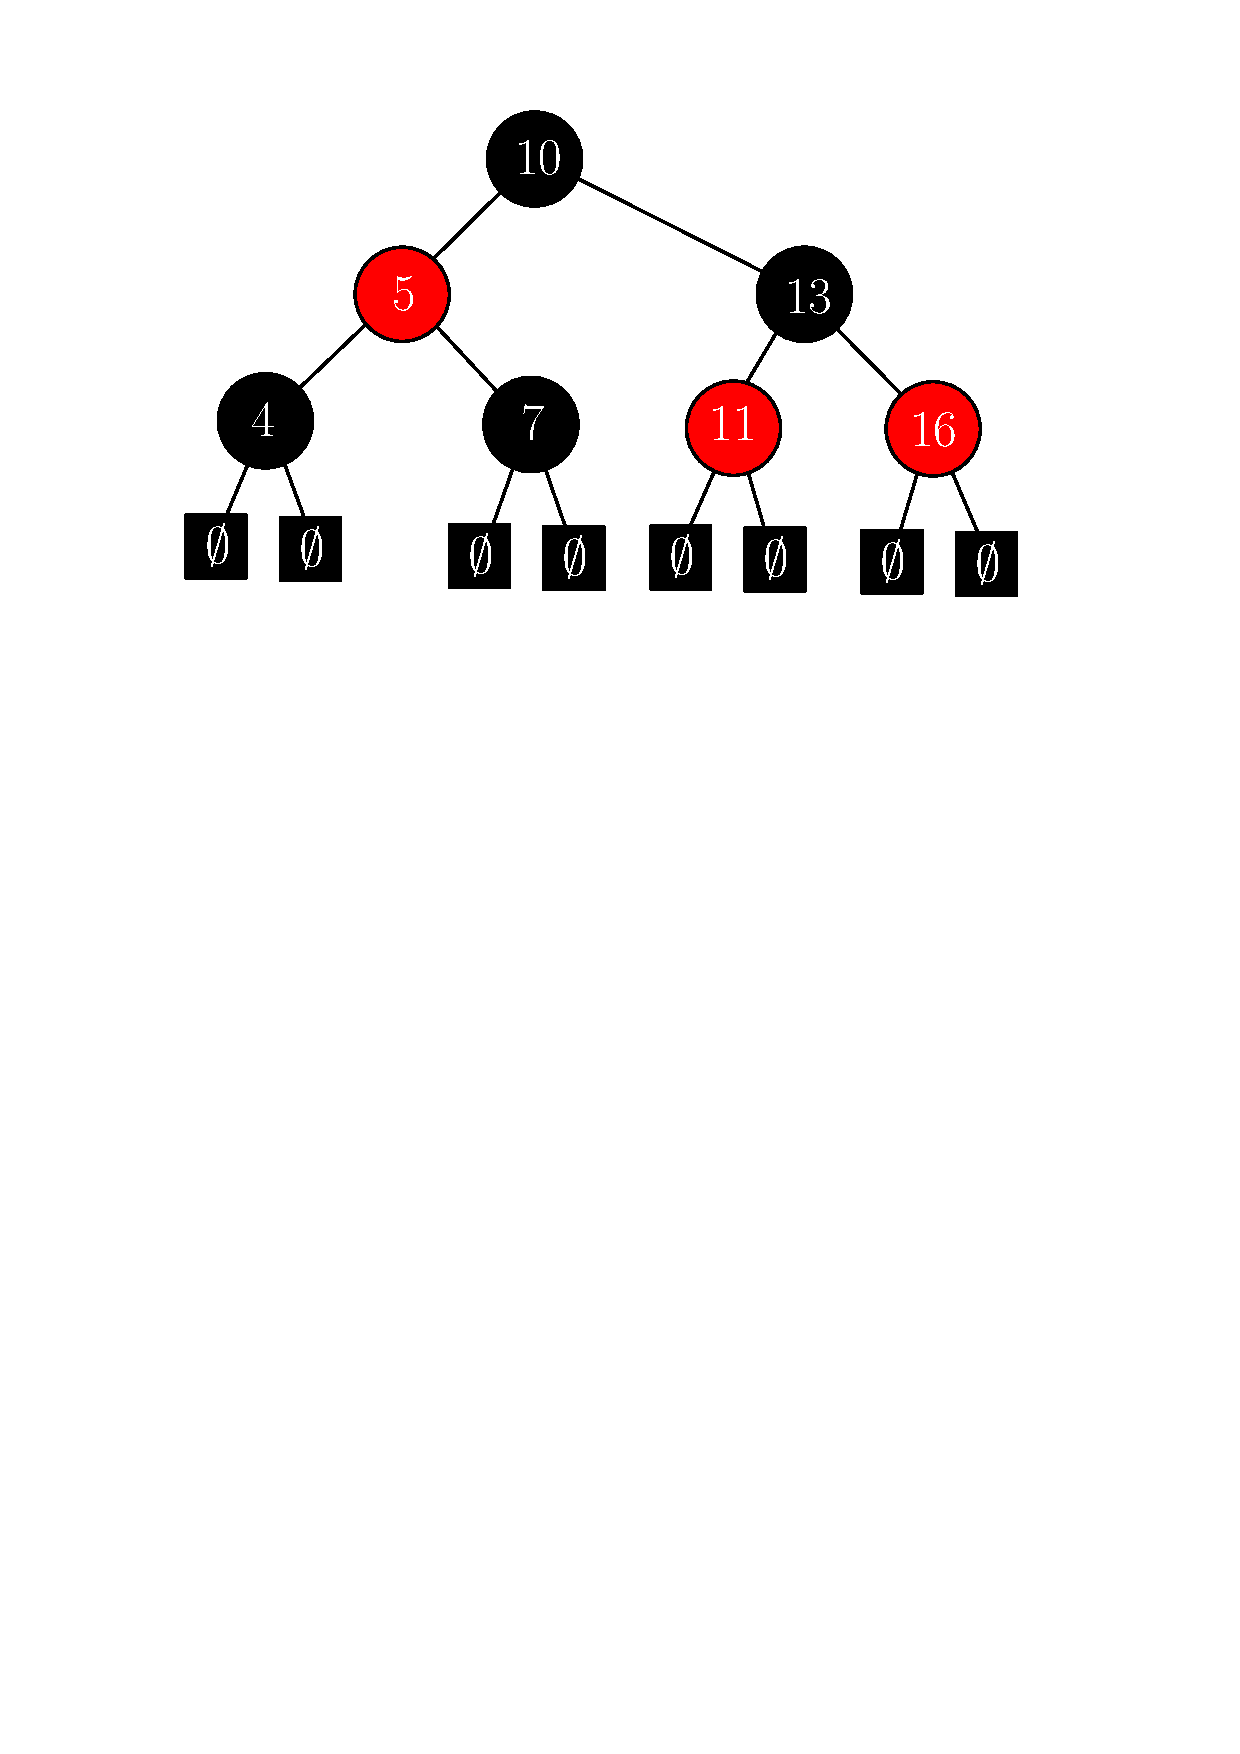
\includegraphics[height=50mm]{./images/redblack1.pdf}
	\end{center}
\end{frame}

\begin{frame}\frametitle{\mytitle}
	\begin{exampleblock}{Implementation}
		\begin{itemize}
			\item jeder Knoten ben\"otigt ein zus\"atzliches Bit f\"ur die Farbe
			\item wir speichern \emph{einen} zus\"atzlichen Knoten als $\emptyset$-Knoten ab
			\item dessen Elternzeiger ist also \emph{nicht} korrekt gesetzt!
		\end{itemize}
	\end{exampleblock}
\end{frame}

\begin{frame}\frametitle{\mytitle}
	\begin{block}{Lemma}
		Ein red black tree mit $n$ Knoten hat H\"ohe $O(\log n)$.
	\end{block}
	\begin{exampleblock}{Beweis}
		Dies folgt unmittelbar aus {\bf RB4} und {\bf RB5}.
	\end{exampleblock}
\end{frame}

\begin{frame}\frametitle{\mytitle}
	\hfill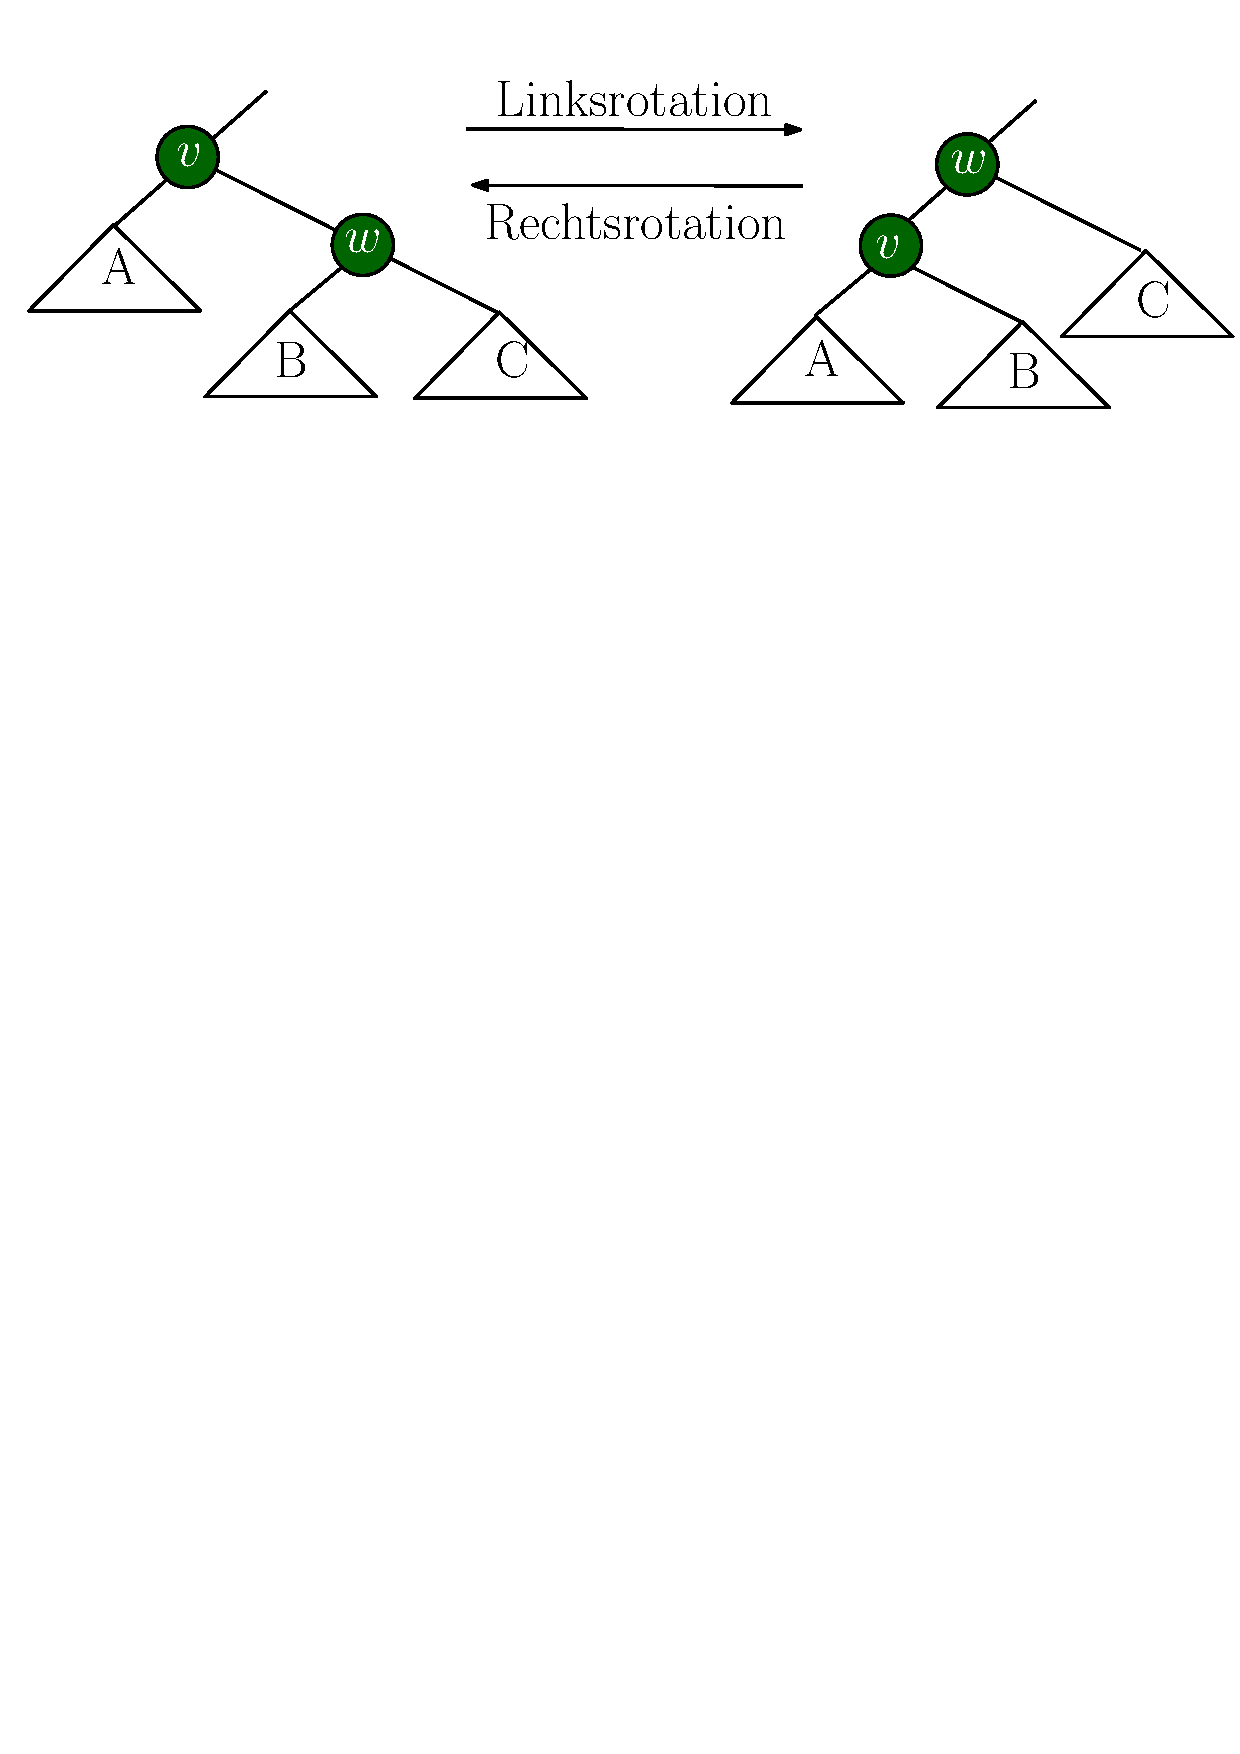
\includegraphics[height=30mm]{./images/rotate1.pdf}
	\begin{exampleblock}{Rotationen}
		\begin{description}
			\item[Linksrotation] um einen Knoten $v$
			\item[Rechtsrotation] um einen Knoten $w$
		\end{description}
	\end{exampleblock}
\end{frame}

\begin{frame}\frametitle{\mytitle}
	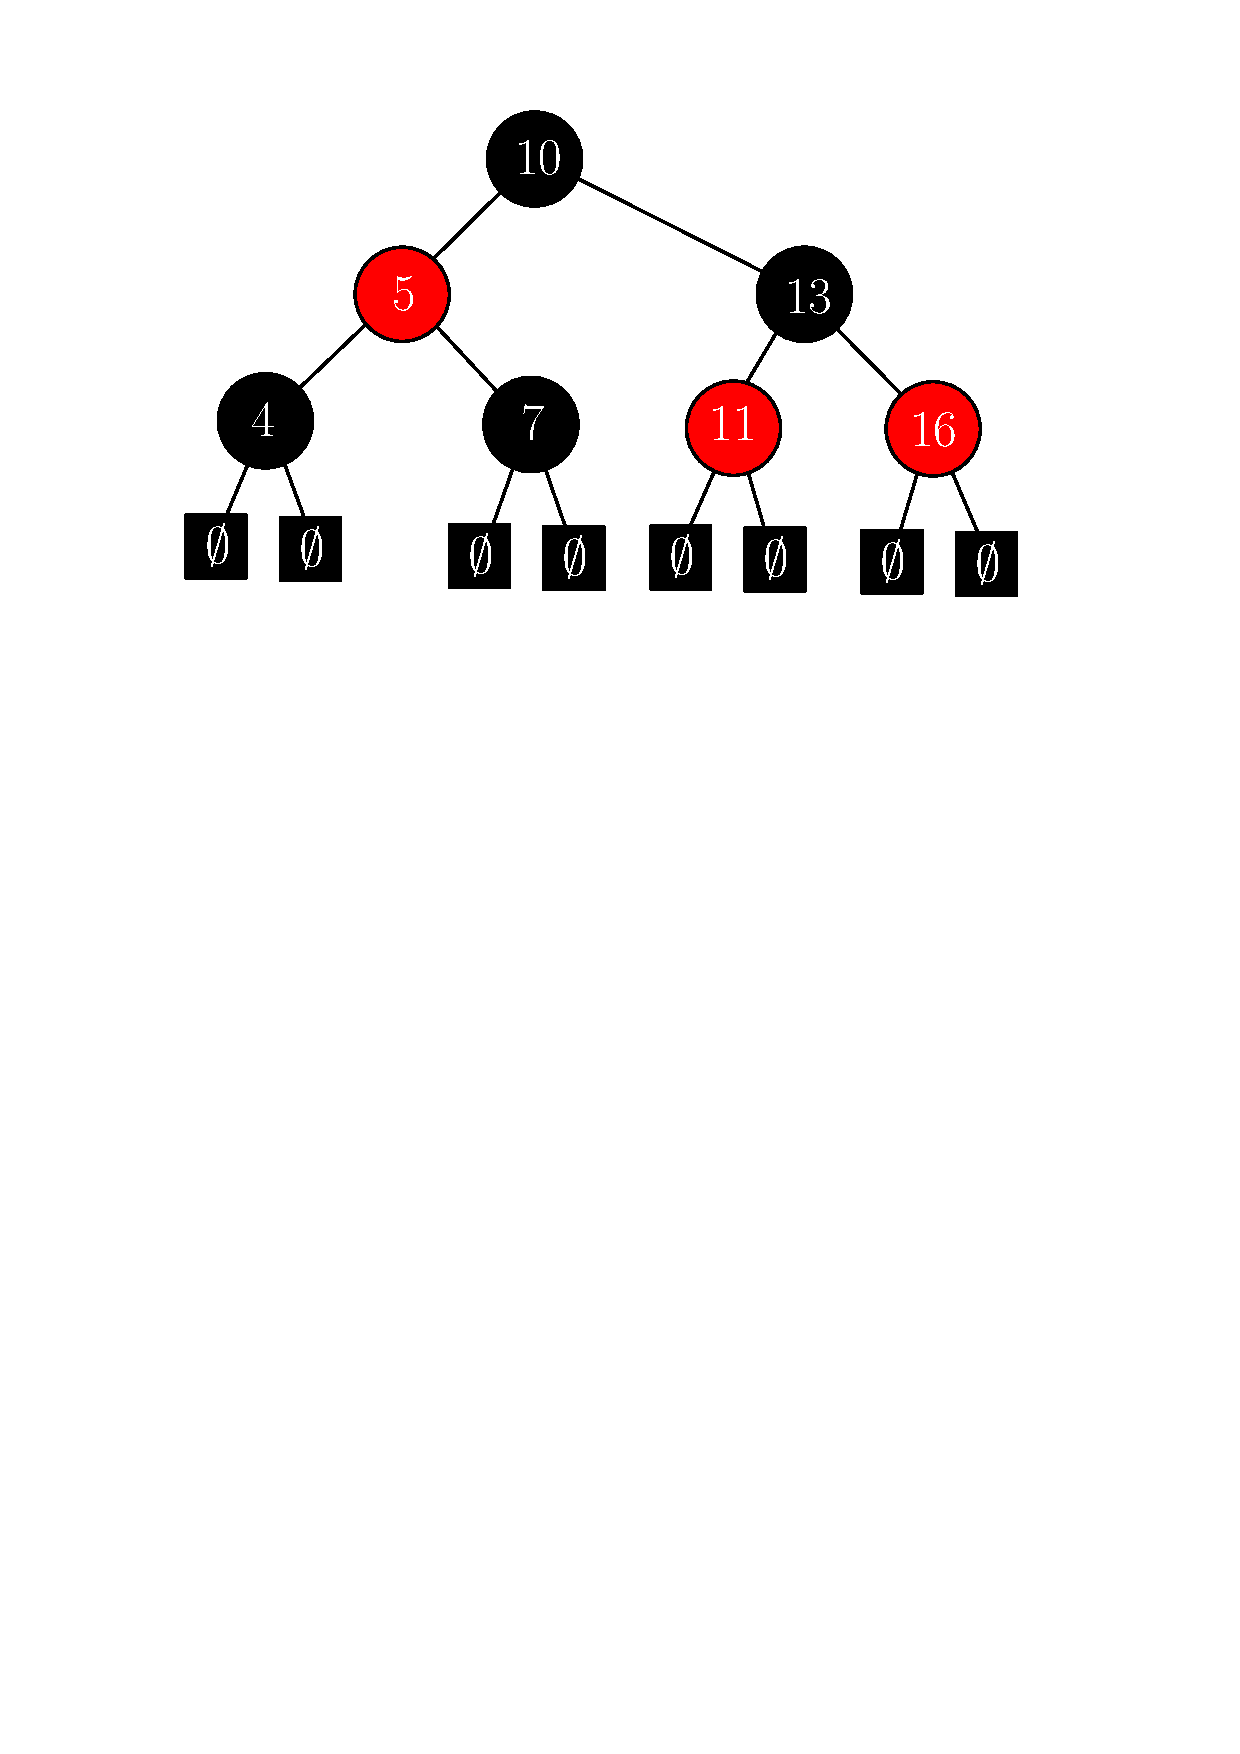
\includegraphics[height=30mm]{./images/redblack1.pdf}
	\hfill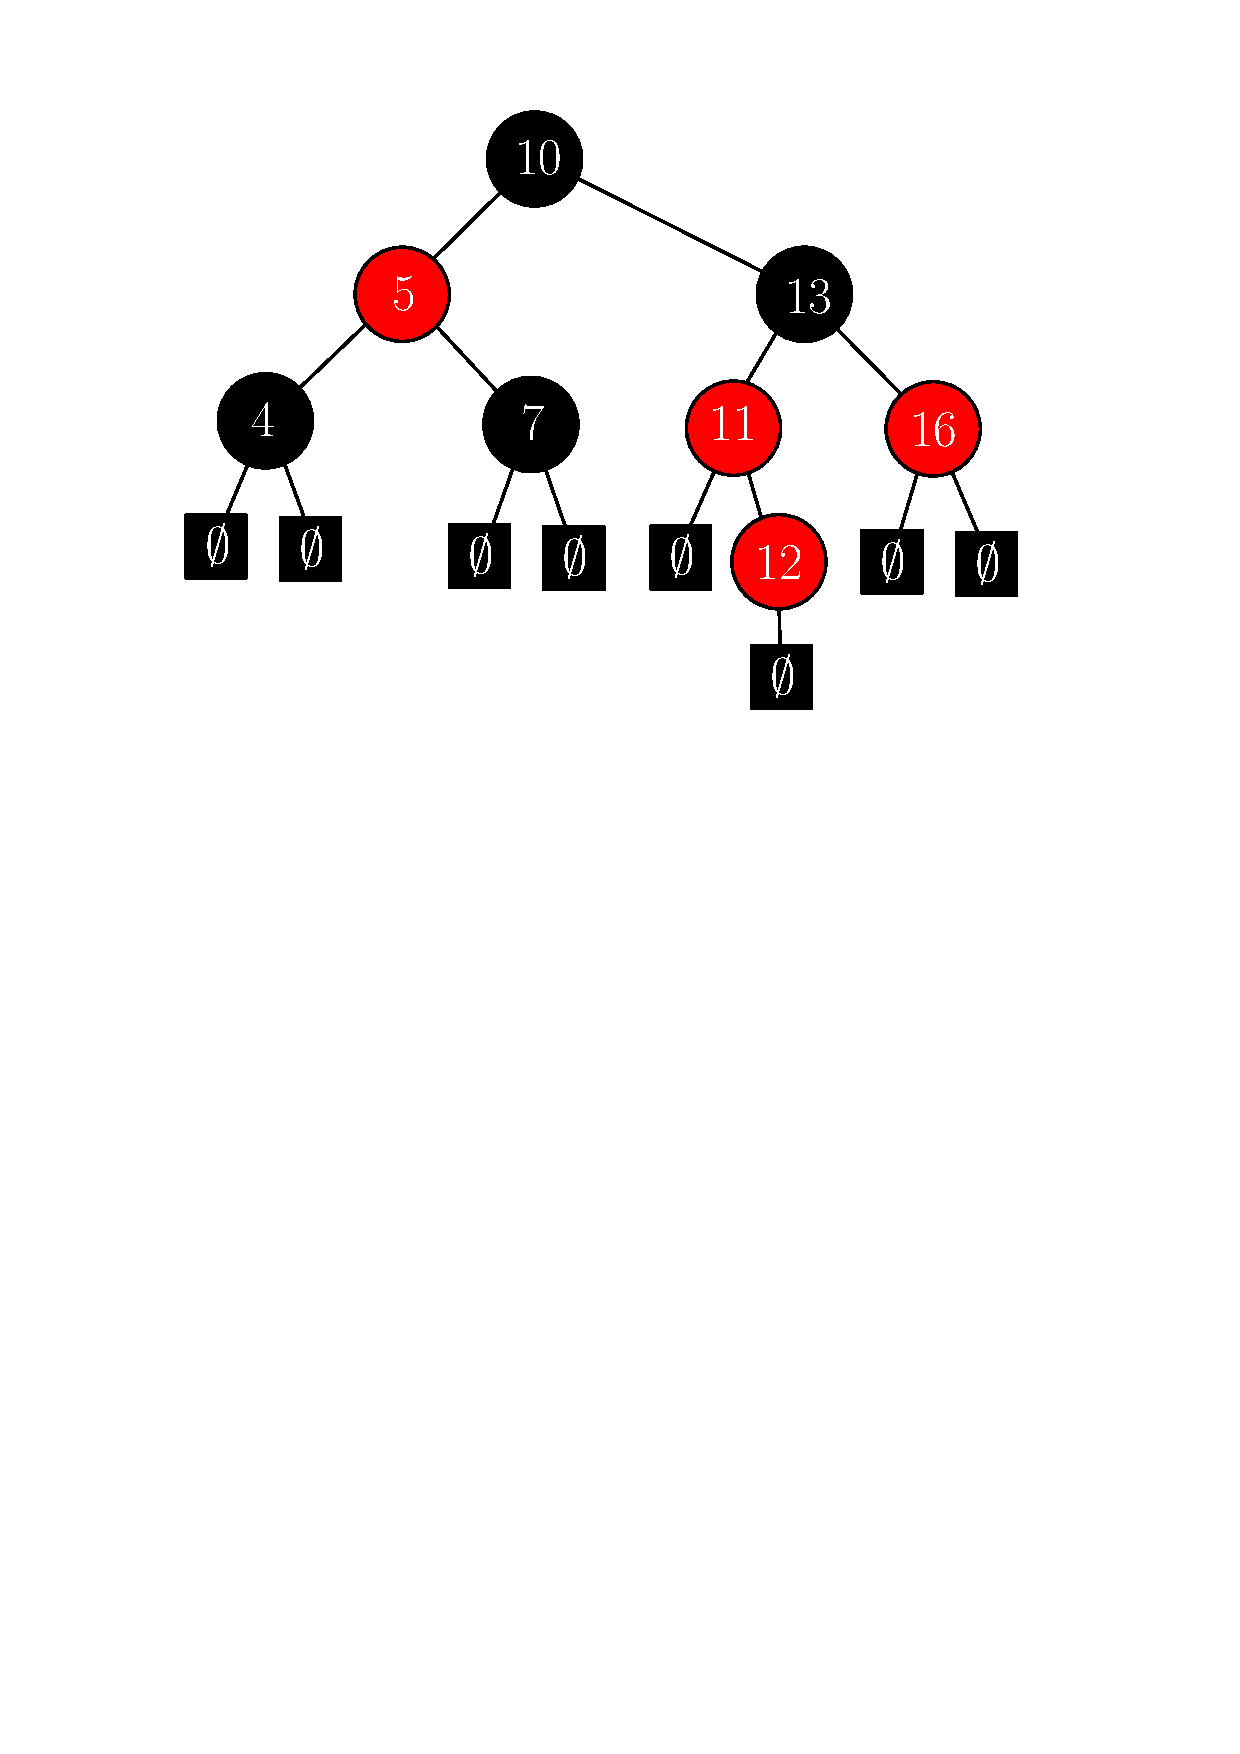
\includegraphics[height=30mm]{./images/redblack2.pdf}
	\begin{exampleblock}{{\tt Insert}: Einf\"ugen eines neuen Knotens}
		\begin{itemize}
			\item zun\"achst verfahren wir genau wie bei ``gew\"ohnlichen'' bin\"aren Suchb\"aumen
			\item der neue Knoten wird rot gef\"arbt
			\item die $\emptyset$-pointer werden auf das $\emptyset$-Objekt gesetzt
			\item \alert{Vorsicht:} RB2 oder RB4 k\"onnten verletzt sein!
		\end{itemize}
	\end{exampleblock}
\end{frame}

\begin{frame}\frametitle{\mytitle}
	\begin{exampleblock}{Wiederherstellen von RB2 und RB4}
		\begin{itemize}
			\item solange der Elternknoten des eingef\"ugten Knotens $v$ rot, ist, betrachten wir drei F\"alle
			\item \alert{Fall 1:} die ``Tante'' $w$ von $v$ ist rot
			\item \alert{Fall 2:} $w$ ist schwarz und $v$ ist ein rechtes Kind
			\item \alert{Fall 3:} $w$ ist schwarz und $v$ ist ein linkes Kind
		\end{itemize}
		\itshape die drei F\"alle lassen sich am besten anhand von Beispielen erkl\"aren; dabei nehmen wir an, da\ss\ der Elternknoten von $v$ ein linkes Kind ist; sonst sind ``links'' und ``rechts'' jeweils zu vertauschen!
	\end{exampleblock}
\end{frame}

\begin{frame}\frametitle{\mytitle}
	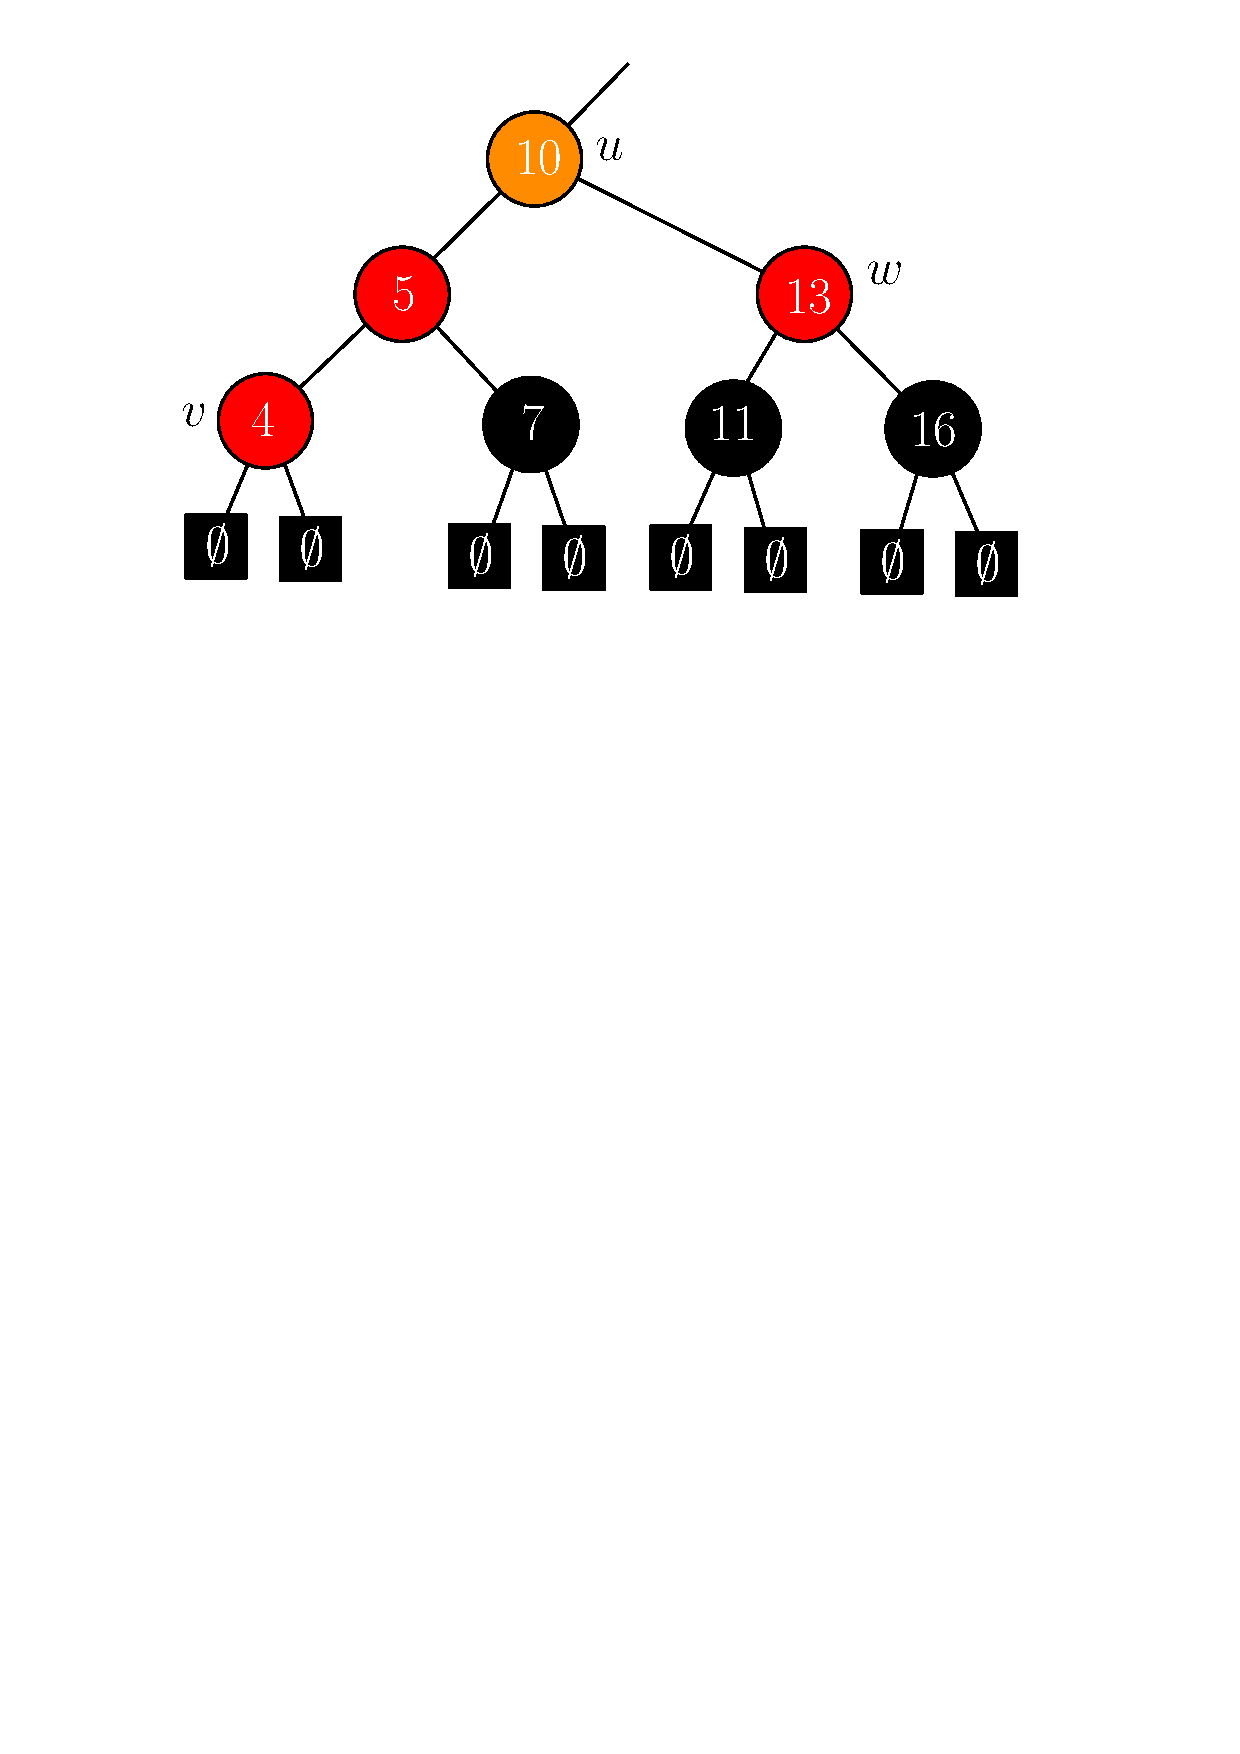
\includegraphics[height=30mm]{./images/redblack_insert1.pdf}\hfill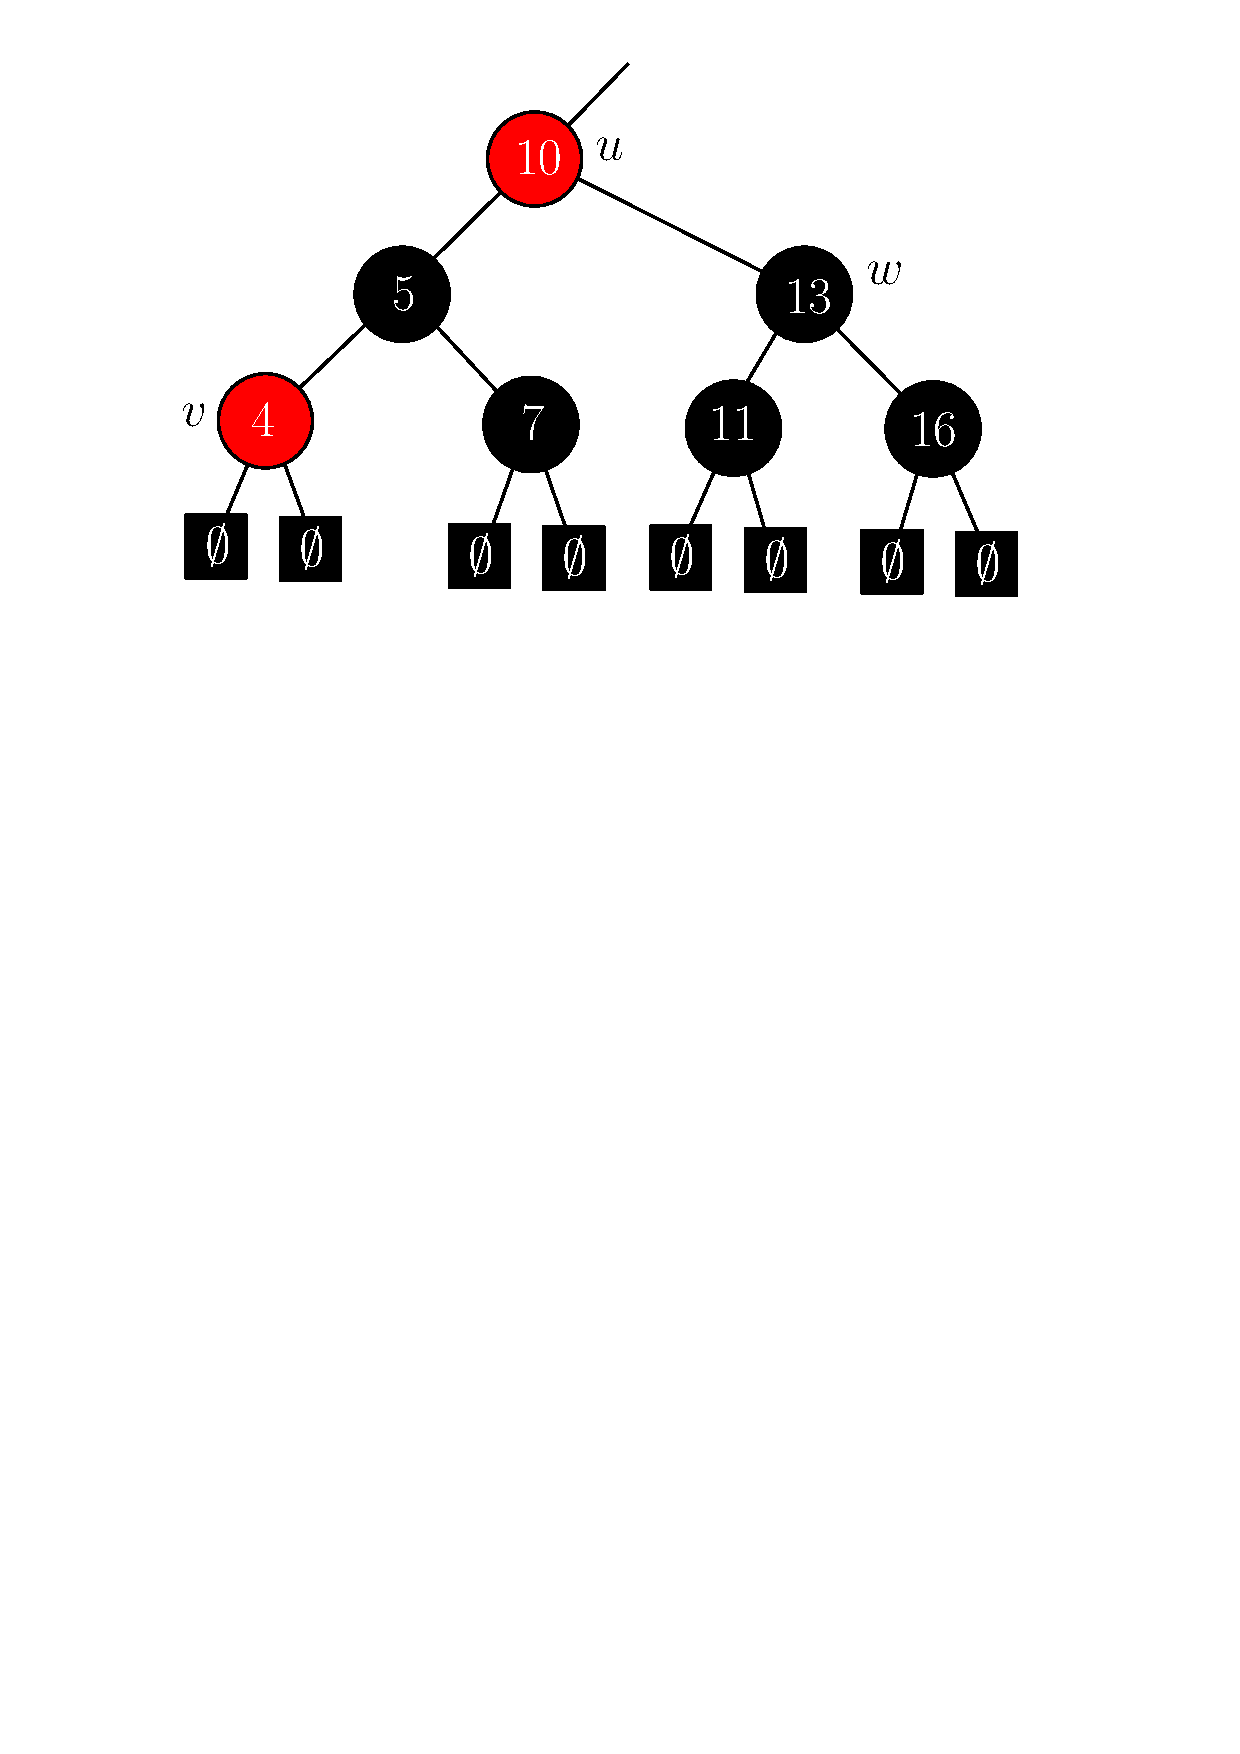
\includegraphics[height=30mm]{./images/redblack_insert1a.pdf}
	\begin{exampleblock}{Fall 1: roter Elternknoten und rote Tante}
		\begin{itemize}
			\item f\"arbe Elternknoten und die Tante schwarz
			\item f\"arbe den Gro\ss elternknoten $u$ rot
			\item f\"uhre die Wiederherstellung rekursiv f\"ur $u$ aus
		\end{itemize}
	\end{exampleblock}
\end{frame}

\begin{frame}\frametitle{\mytitle}
	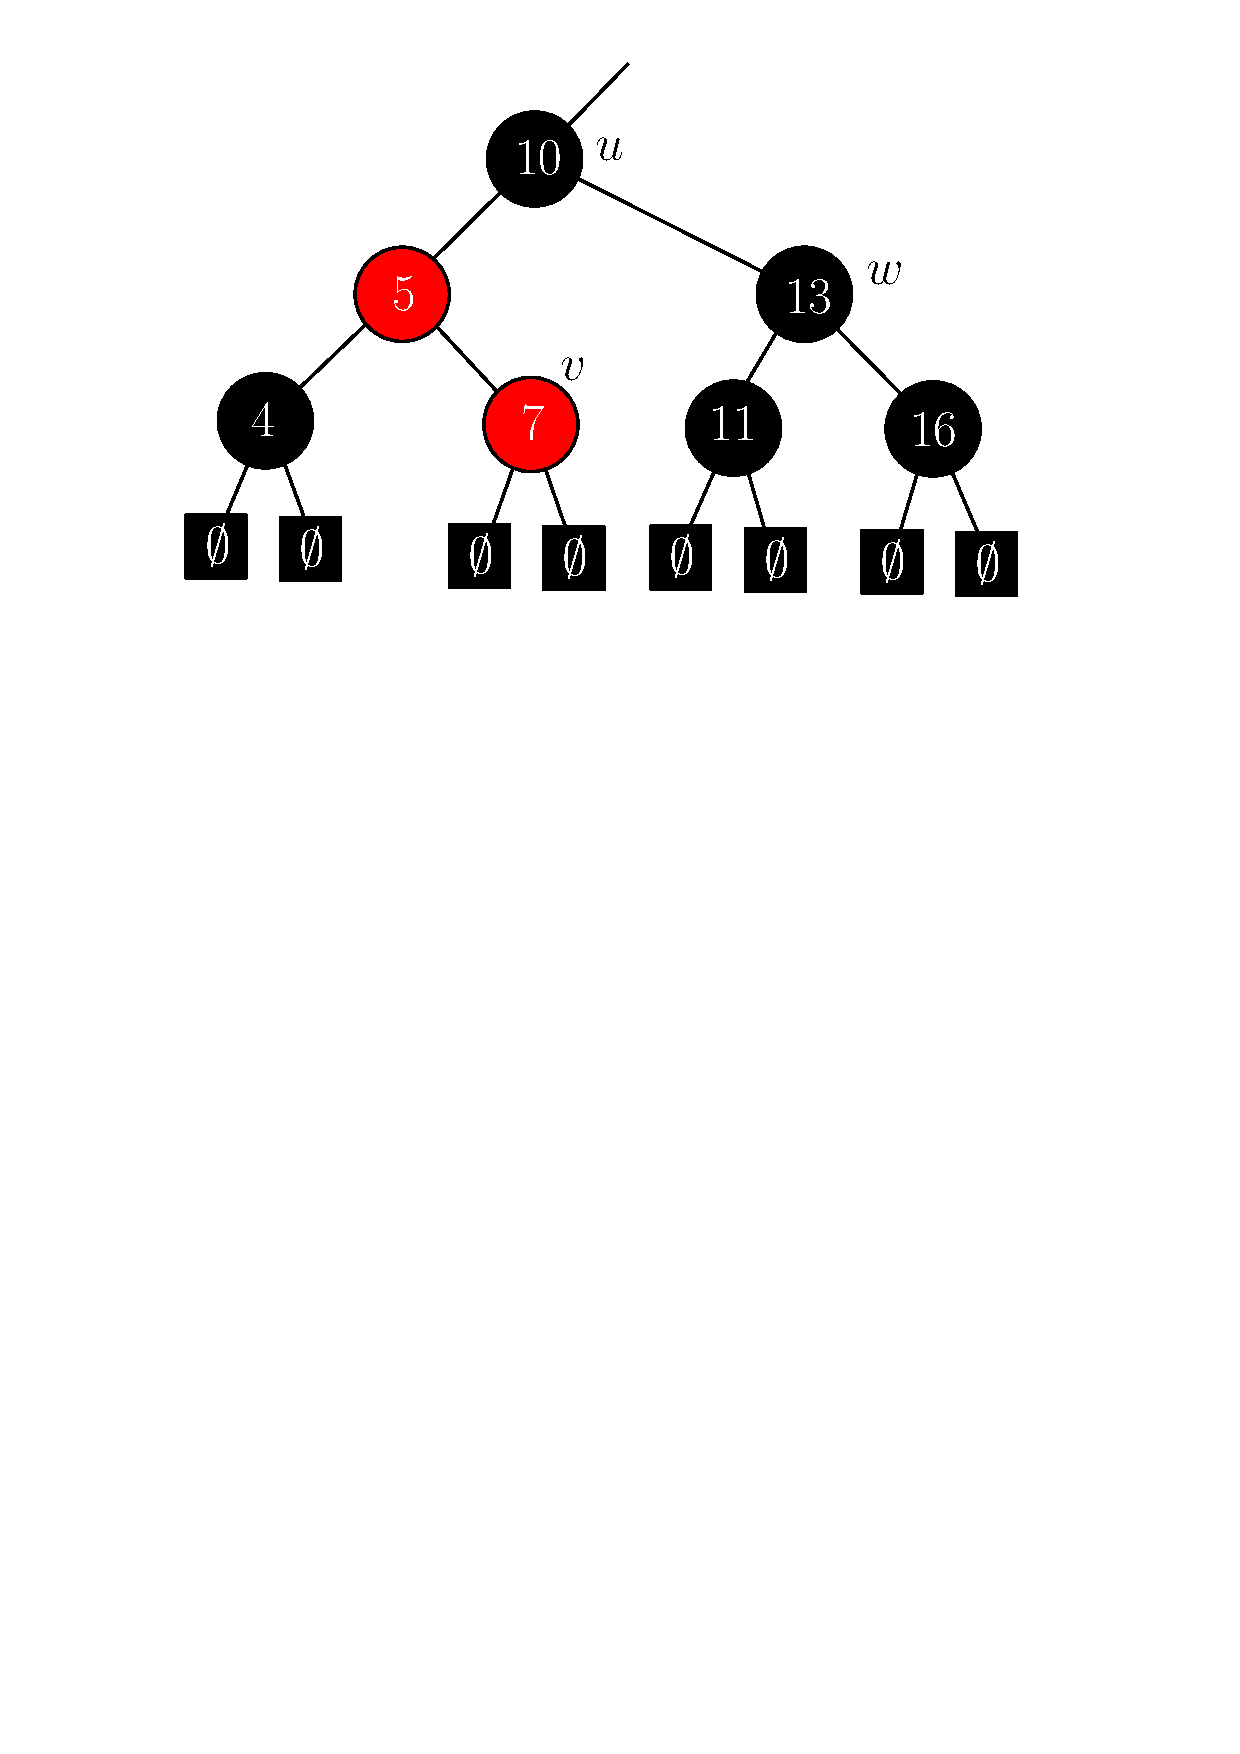
\includegraphics[height=30mm]{./images/redblack_insert2.pdf}\hfill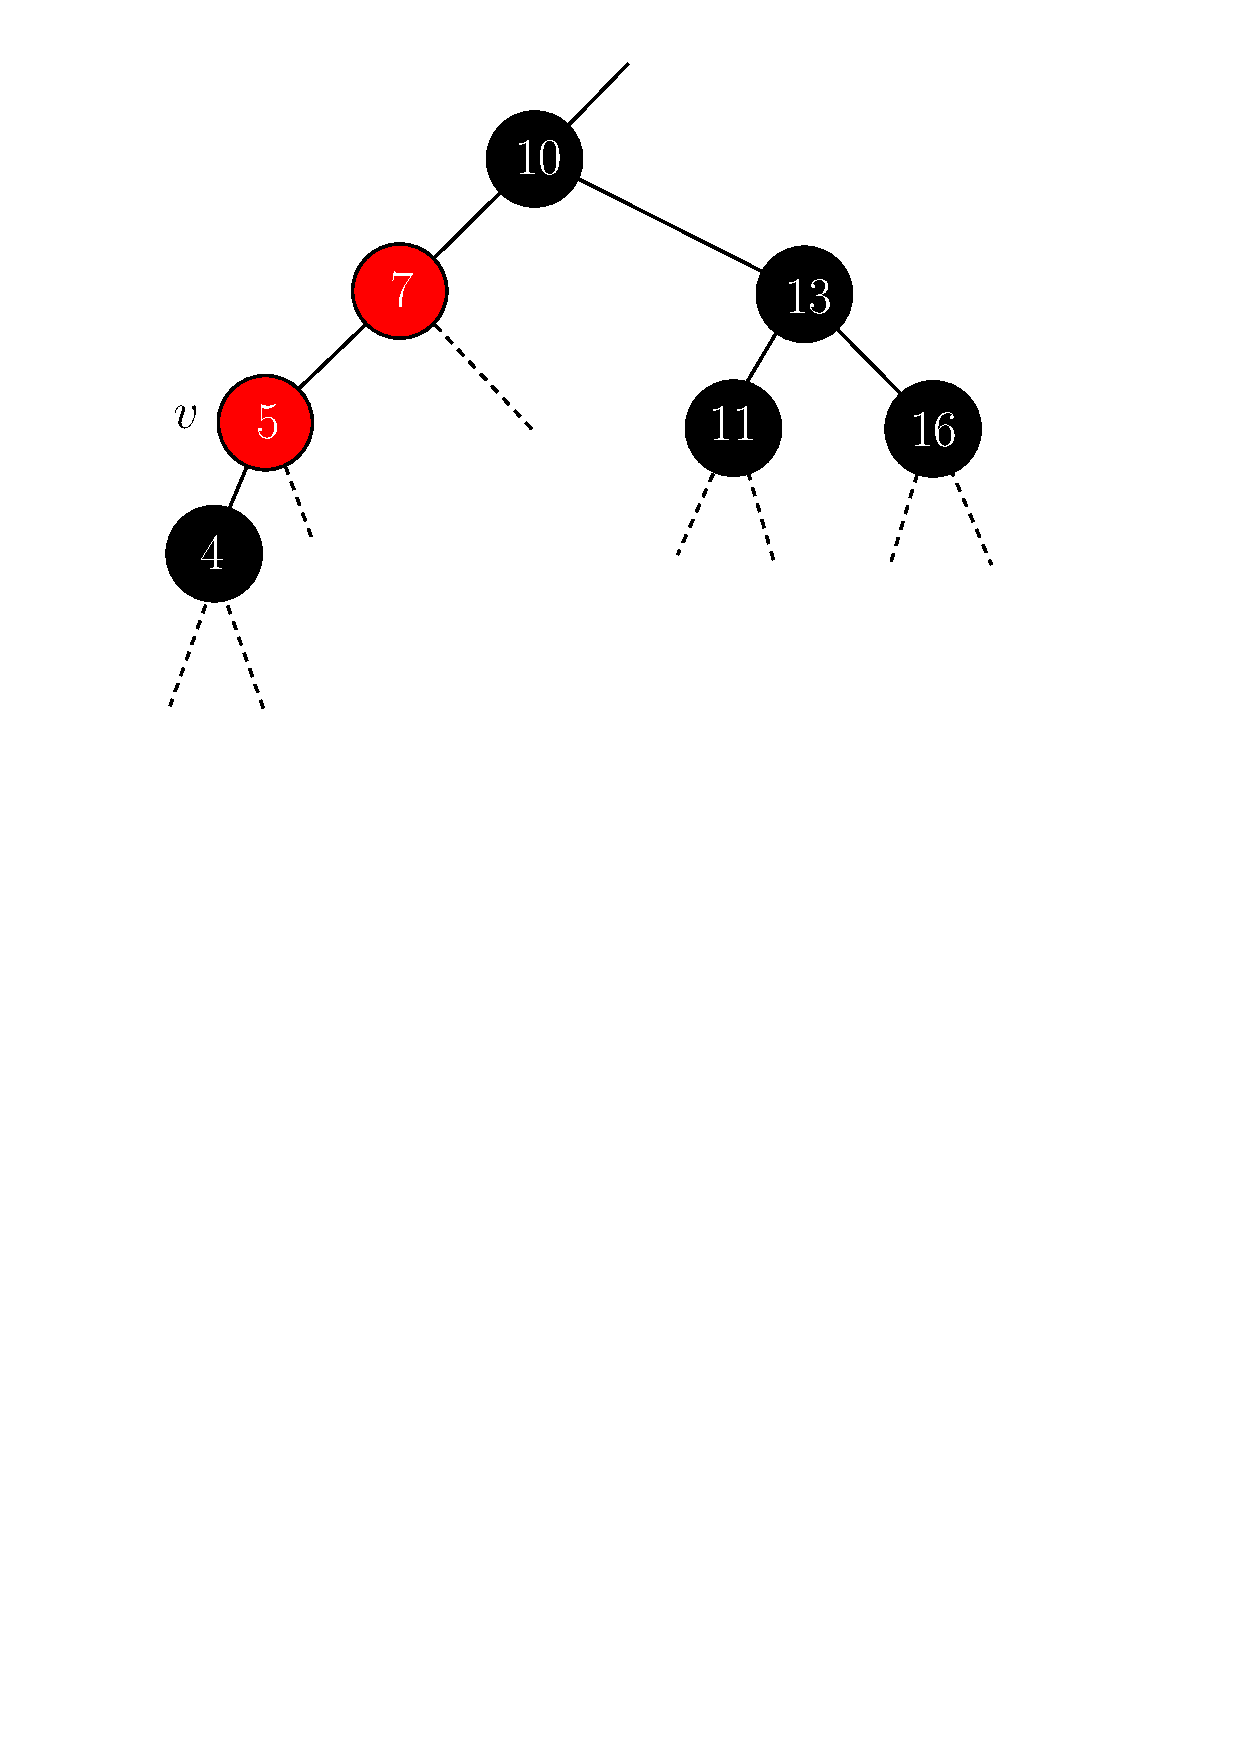
\includegraphics[height=30mm]{./images/redblack_insert2a.pdf}
	\begin{exampleblock}{Fall 2: roter Elternknoten, schwarze Tante, rechtes Kind}
		\begin{itemize}
			\item f\"uhre eine Linksrotation um $v$ durch
			\item weiter mit Fall 3
		\end{itemize}
	\end{exampleblock}
\end{frame}

\begin{frame}\frametitle{\mytitle}
	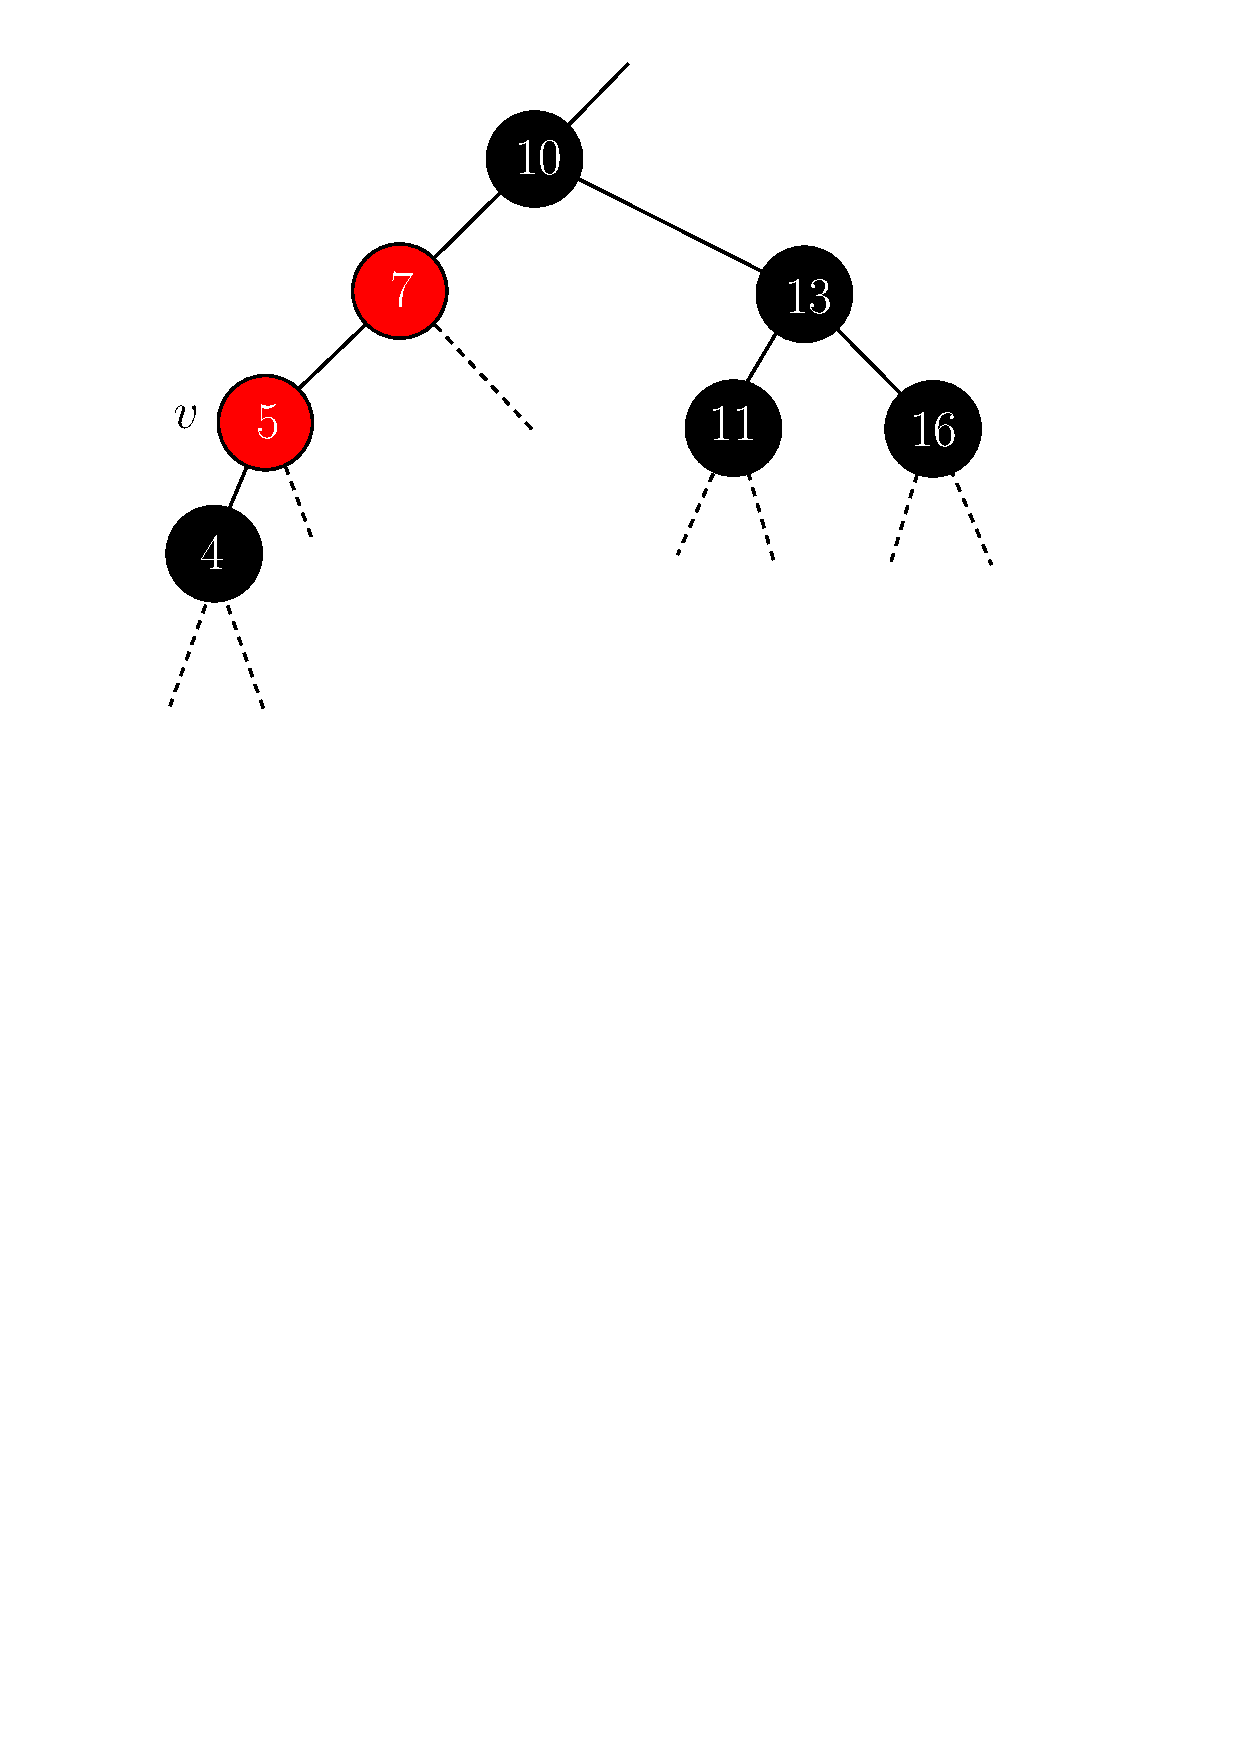
\includegraphics[height=30mm]{./images/redblack_insert2a.pdf}\hfill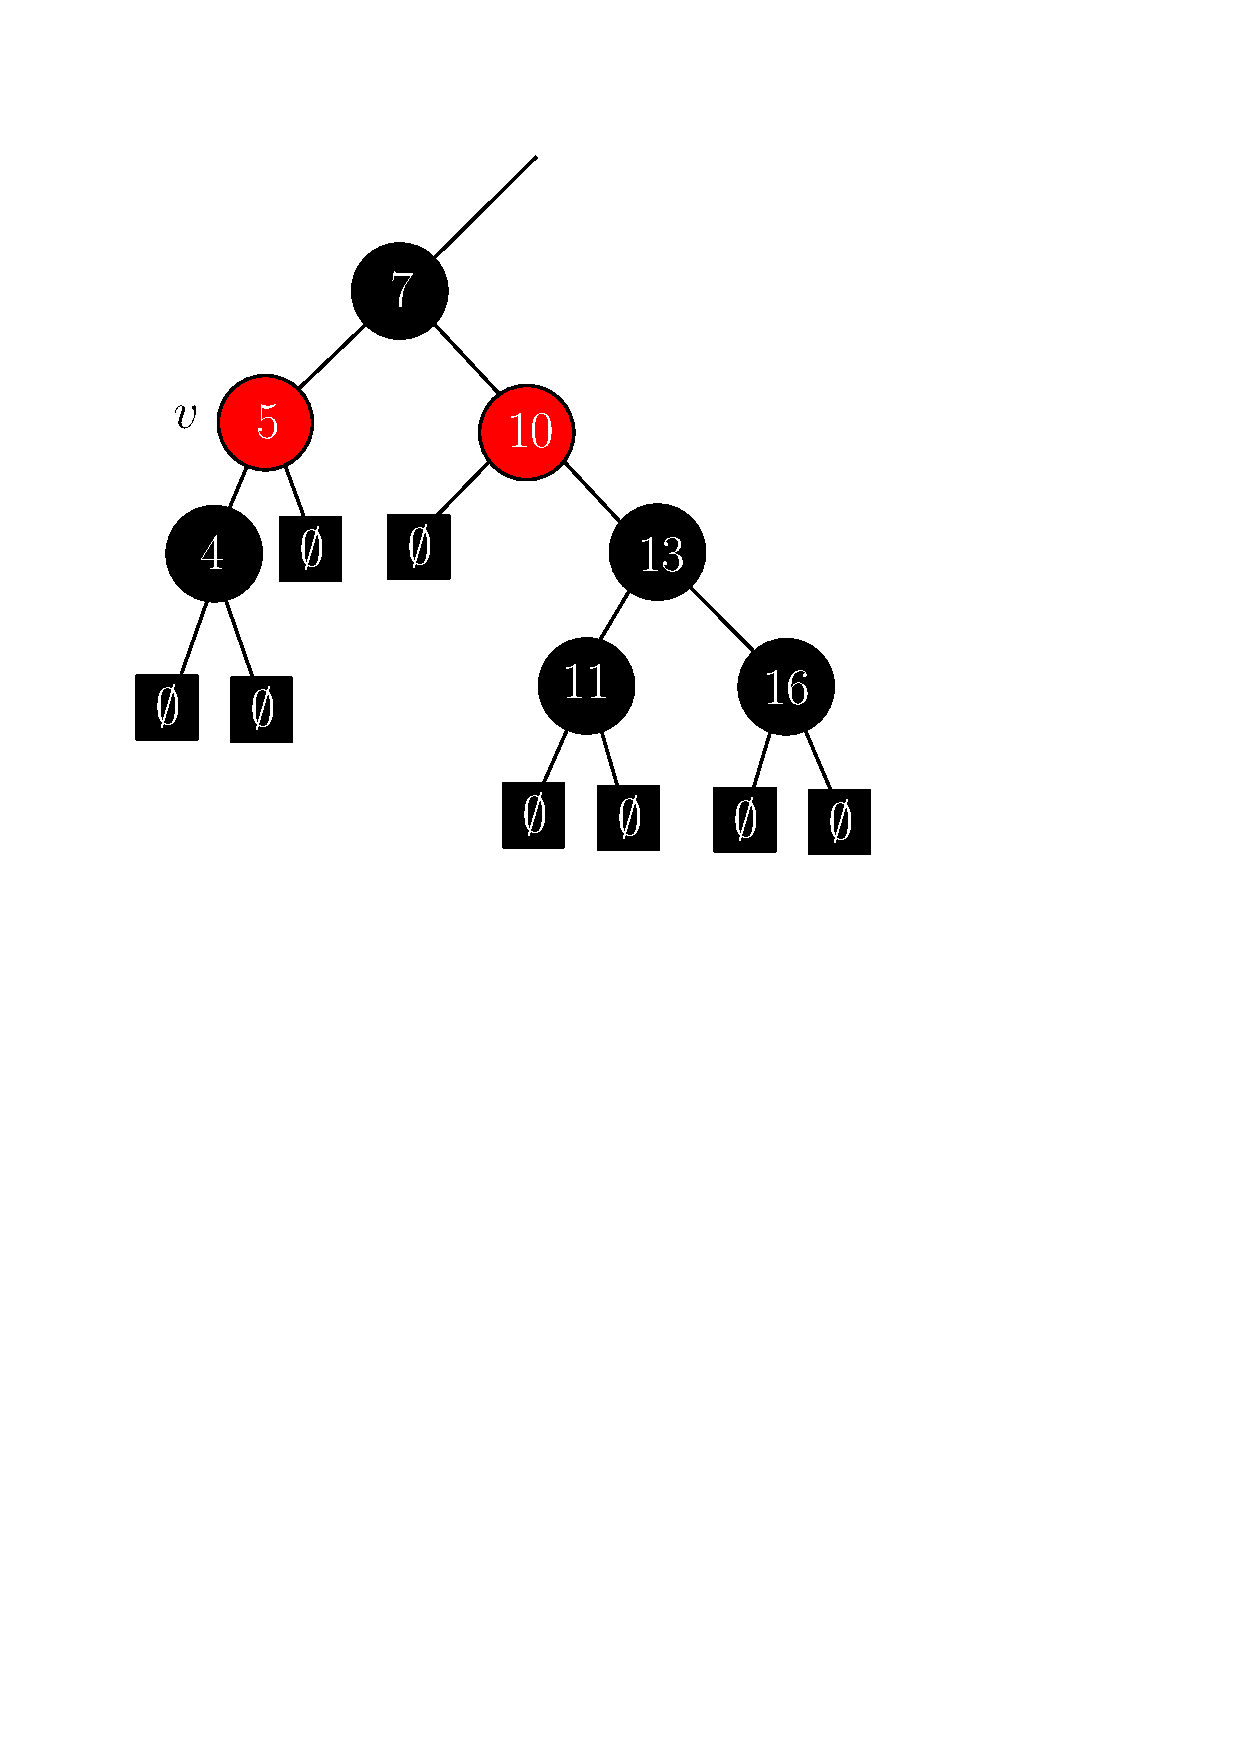
\includegraphics[height=30mm]{./images/redblack_insert3a.pdf}
	\begin{exampleblock}{Fall 3: roter Elternknoten, schwarze Tante, linkes Kind}
		\begin{itemize}
			\item f\"arbe den Elternknoten von $v$ schwarz und den Gro\ss elternknoten $u$ rot
			\item dann Rechtsrotation um den Gro\ss elternknoten $u$
		\end{itemize}
	\end{exampleblock}
\end{frame}

\begin{frame}\frametitle{\mytitle}
	\begin{exampleblock}{Abschlu\ss\ Wiederherstellung}
		\begin{itemize}
			\item am Ende der Wiederherstellungsoperation wird die Wurzel schwarz gef\"arbt
			\item dadurch wird RB2 garantiert
		\end{itemize}
	\end{exampleblock}
\end{frame}

\begin{frame}\frametitle{\mytitle}
	\begin{block}{Proposition}
Die Einf\"ugeoperation inkl.\ Wiederherstellung hat Laufzeit $O(\log n)$ und stellt die Eigenschaften RB1--RB5 her.
	\end{block}
\begin{exampleblock}{Beweis}
		\begin{itemize}
			\item in den F\"allen 2 und 3 ist die Gesamtlaufzeit $O(1)$
			\item in Fall 1 bewegt sich $v$ auf die Wurzel zu
			\item wir stoppen also nach $O(\log n)$ Schritten
		\end{itemize}
	\end{exampleblock}
\end{frame}

\begin{frame}\frametitle{\mytitle}
	\begin{overprint}
		\onslide<1>
		\begin{exampleblock}{Entfernen eines Knotens $z$}
			\begin{itemize}
				\item verfahre wie beim L\"oschen von $z$ in einem bin\"aren Suchbaum
				\item sei $y$ der Knoten, der die Stelle von $z$ einnimmt
				\item $y$ \"ubernimmt die Farbe von $z$
				\item sei $v$ das Kind von $y$, bzw.\ $\emptyset$, falls $y$ kein Kind hat
				\item \itshape dabei identifizieren wir $\emptyset$ mit dem $\emptyset$-Objekt des Baums
			\end{itemize}
		\end{exampleblock}
		\onslide<2>
		\begin{exampleblock}{Wenn $y$ schwarz war, k\"onnen Verletzungen von RB1--RB5 eintreten}
			\begin{itemize}
				\item m\"oglicherweise war $y$ die Wurzel; das Kind $v$ tritt an die Stelle von $y$, wird somit die neue Wurzel, ist aber wom\"oglich rot; also RB2 verletzt
				\item wenn $v$ und der Elternknoten $u$ von $z$ rot sind, ist RB4 verletzt
				\item die Pfade, die vormals $y$ enthalten haben, enthalten jetzt einen schwarzen Knoten weniger; somit RB5 verletzt
				\item wir k\"onnen uns $v$, der an die Stelle von $y$ tritt, als einen ``doppelt schwarzen'' Knoten vorstellen
				\item \itshape wir unterscheiden vier F\"alle, die nach der Farbe des Schwesterknotens $w$ von $v$ und den Farben der Kinder von $w$ unterscheiden
				\item \itshape dabei nehmen wir an, da\ss\ $v$ ein linkes Kind ist; andernfalls sind ``links'' und ``rechts'' zu vertauschen
			\end{itemize}
		\end{exampleblock}
	\end{overprint}
\end{frame}

\begin{frame}\frametitle{\mytitle}
	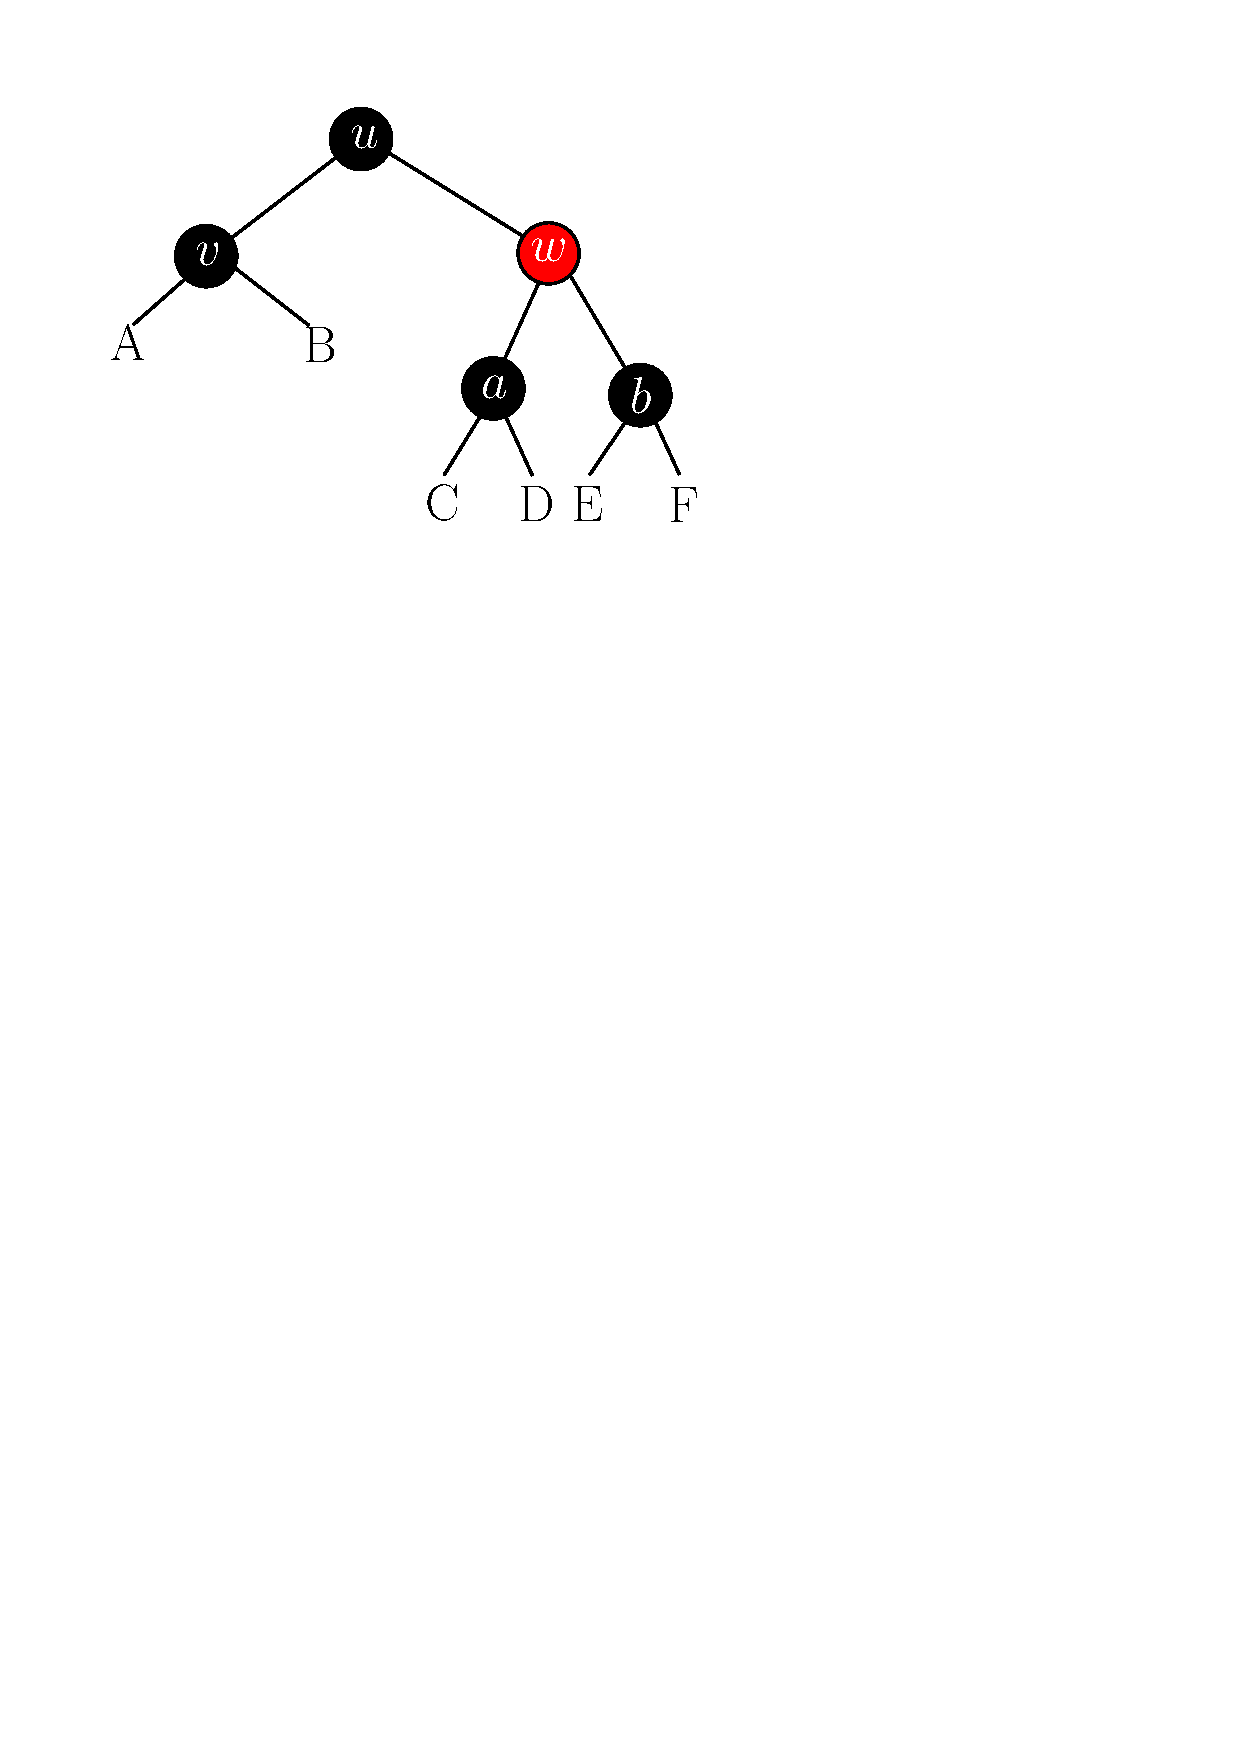
\includegraphics[height=30mm]{./images/rbtree_del_1.pdf}\hfill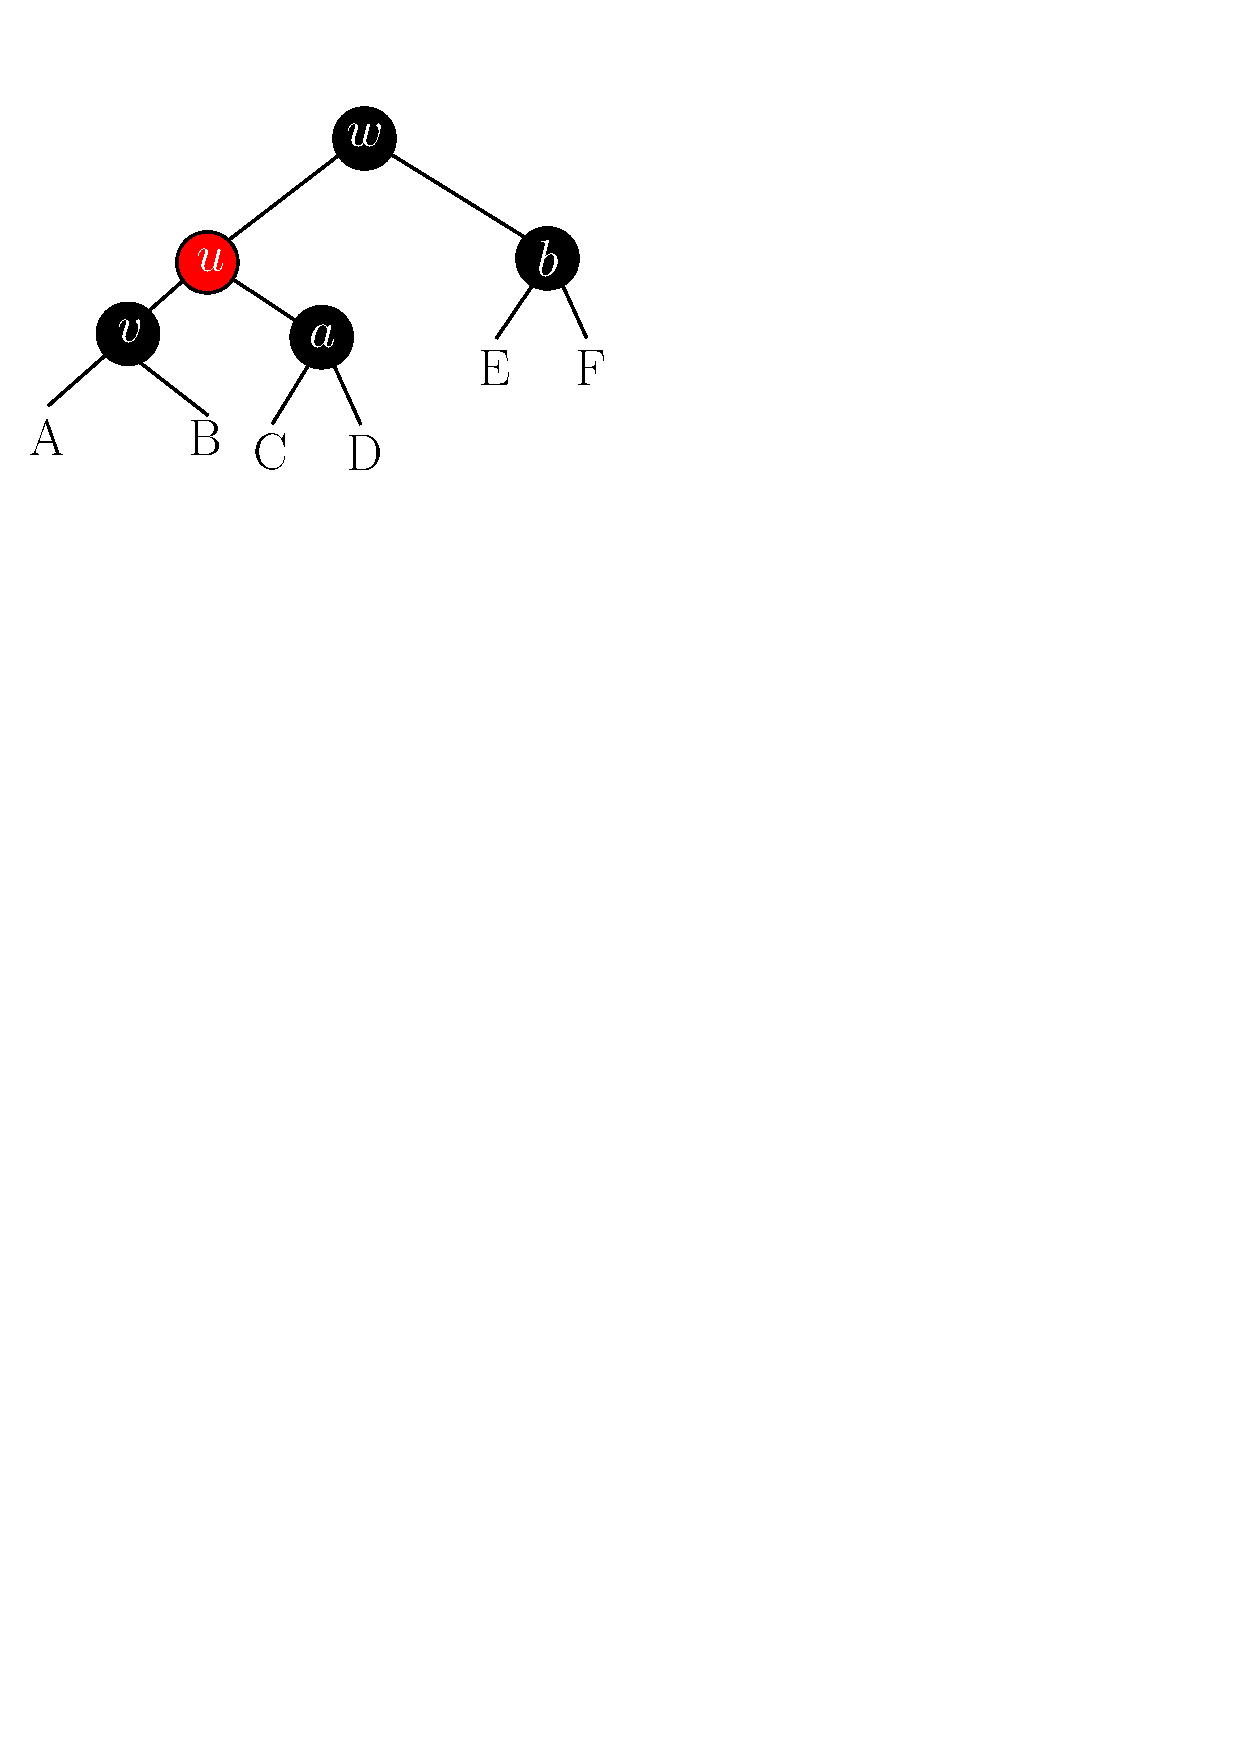
\includegraphics[height=30mm]{./images/rbtree_del_1a.pdf}
	\begin{exampleblock}{Fall 1: roter Schwesterknoten $w$}
		\begin{itemize}
			\item vertausche die Farben von $w$ und $u$
			\item f\"uhre eine Linksrotation um $u$ aus
			\item fahre mit Fall 2/3/4 fort, wobei nun $w=a$ der neue Schwesterknoten ist
		\end{itemize}
	\end{exampleblock}
\end{frame}

\begin{frame}\frametitle{\mytitle}
	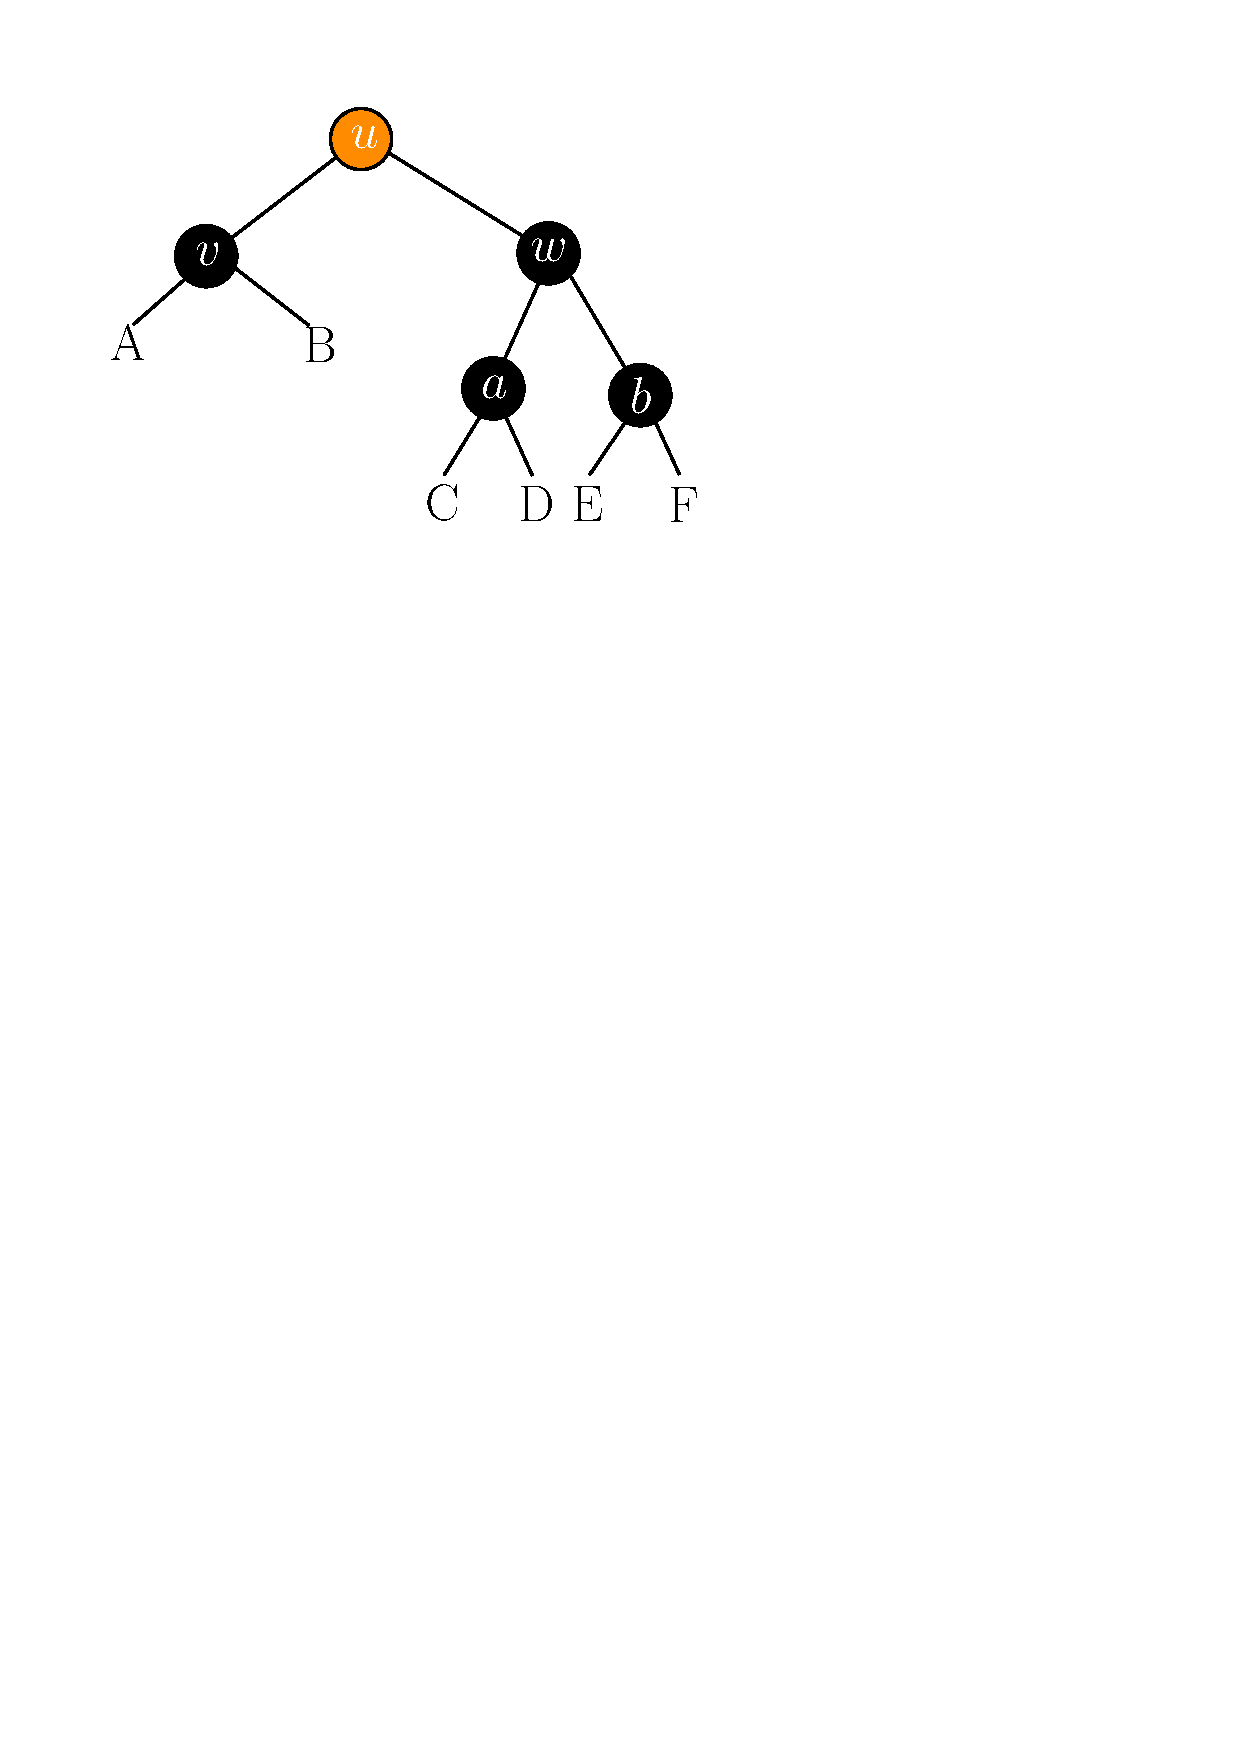
\includegraphics[height=30mm]{./images/rbtree_del_2.pdf}\hfill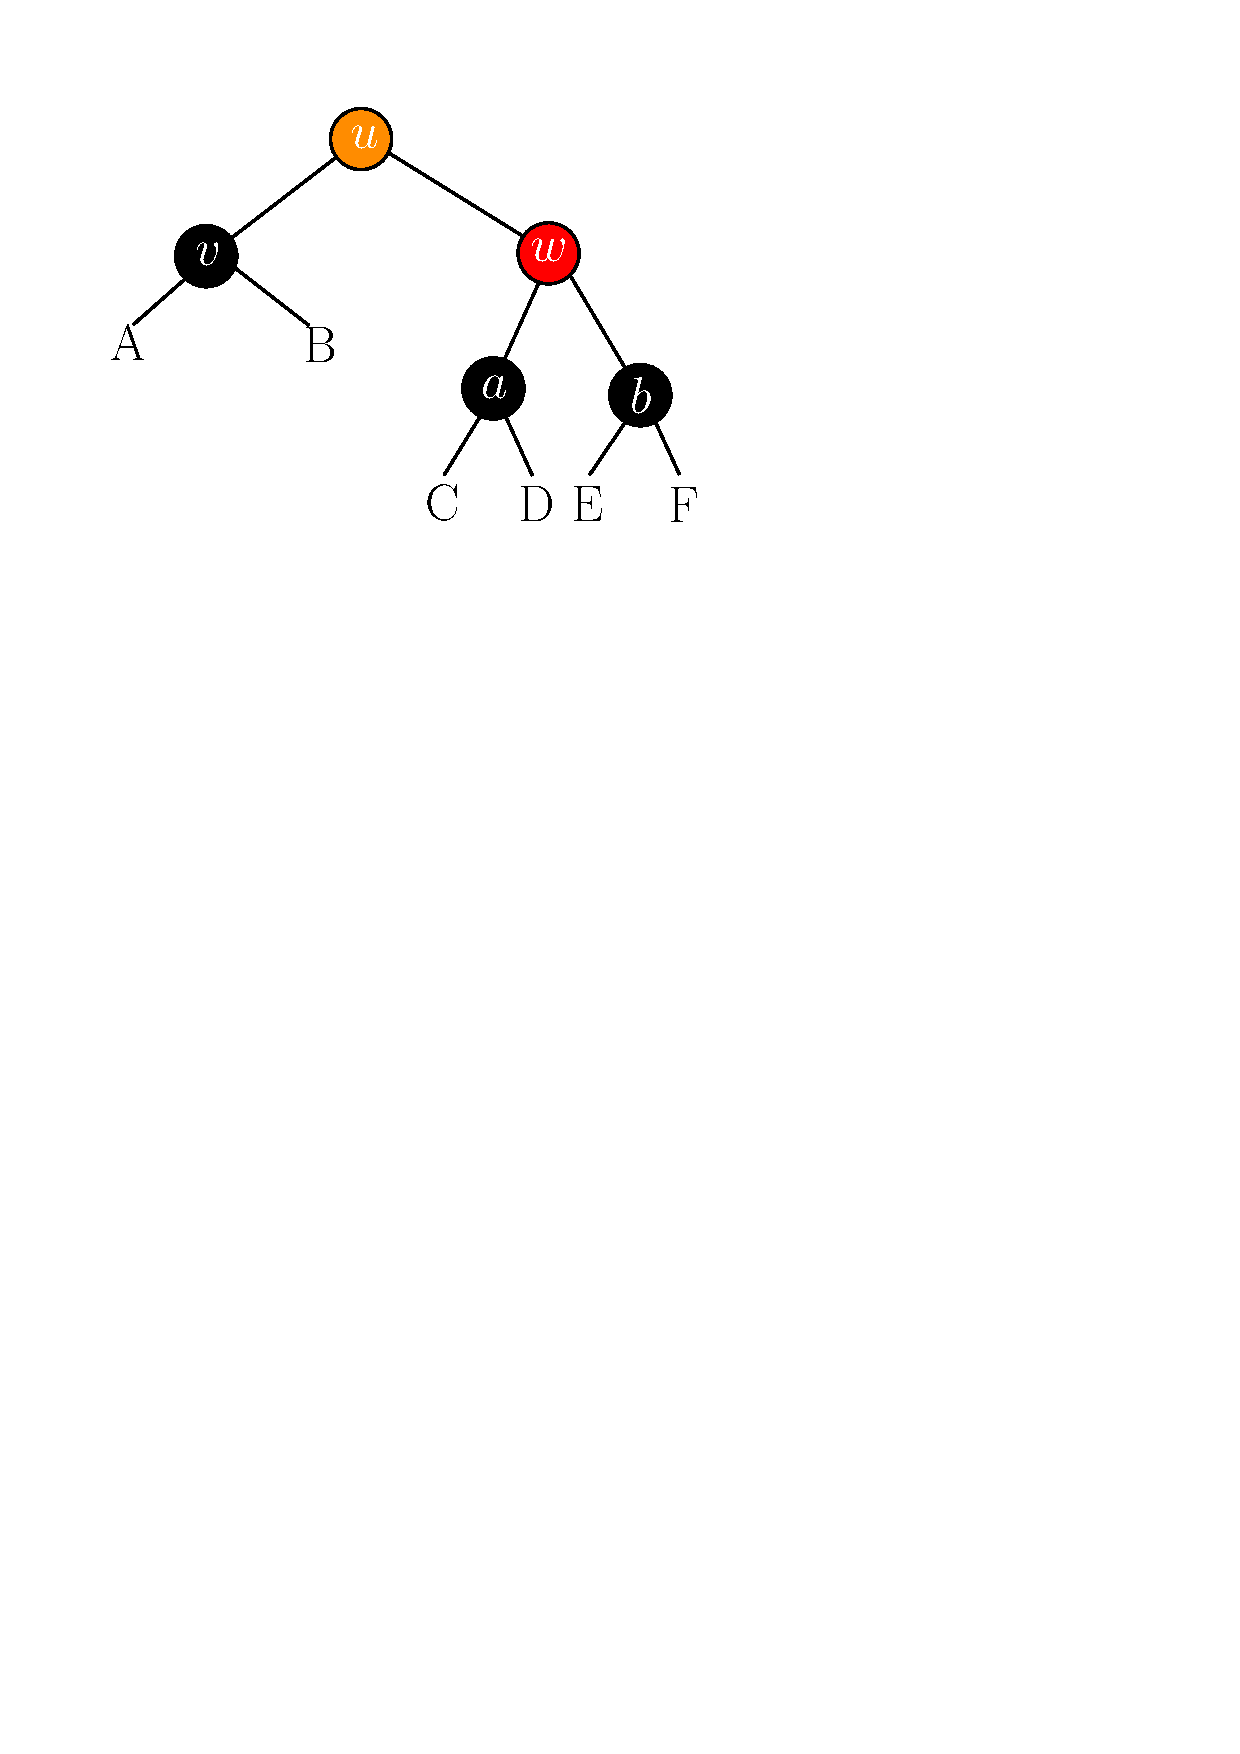
\includegraphics[height=30mm]{./images/rbtree_del_2a.pdf}
	\begin{exampleblock}{Fall 2: schwarzer Schwesterknoten $w$, beide Kinder von $w$ sind schwarz}
		\begin{itemize}
			\item f\"arbe den Schwesterknoten $w$ rot
			\item fahre rekursiv mit $v=u$ fort
			\item (der Knoten $u$ kann rot oder schwarz sein)
		\end{itemize}
	\end{exampleblock}
\end{frame}

\begin{frame}\frametitle{\mytitle}
	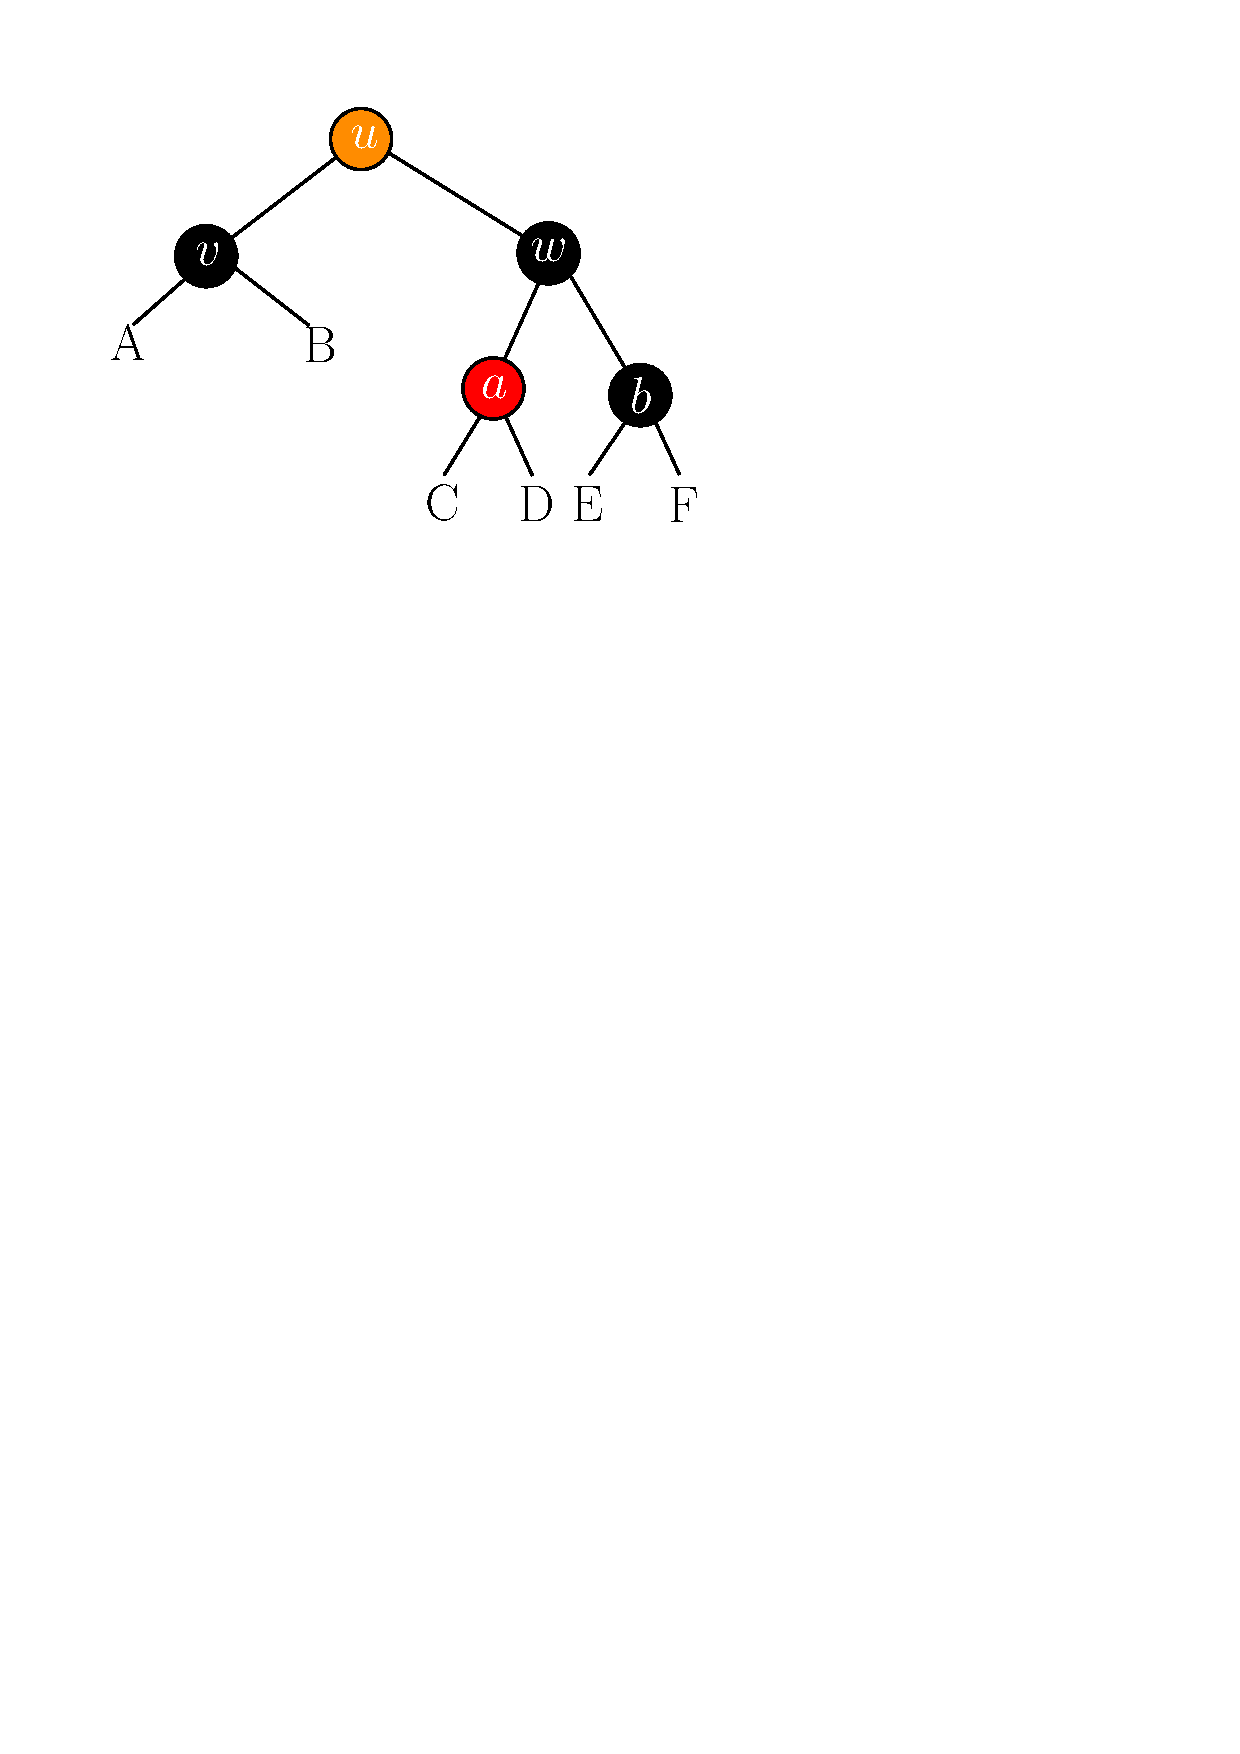
\includegraphics[height=30mm]{./images/rbtree_del_3.pdf}\hfill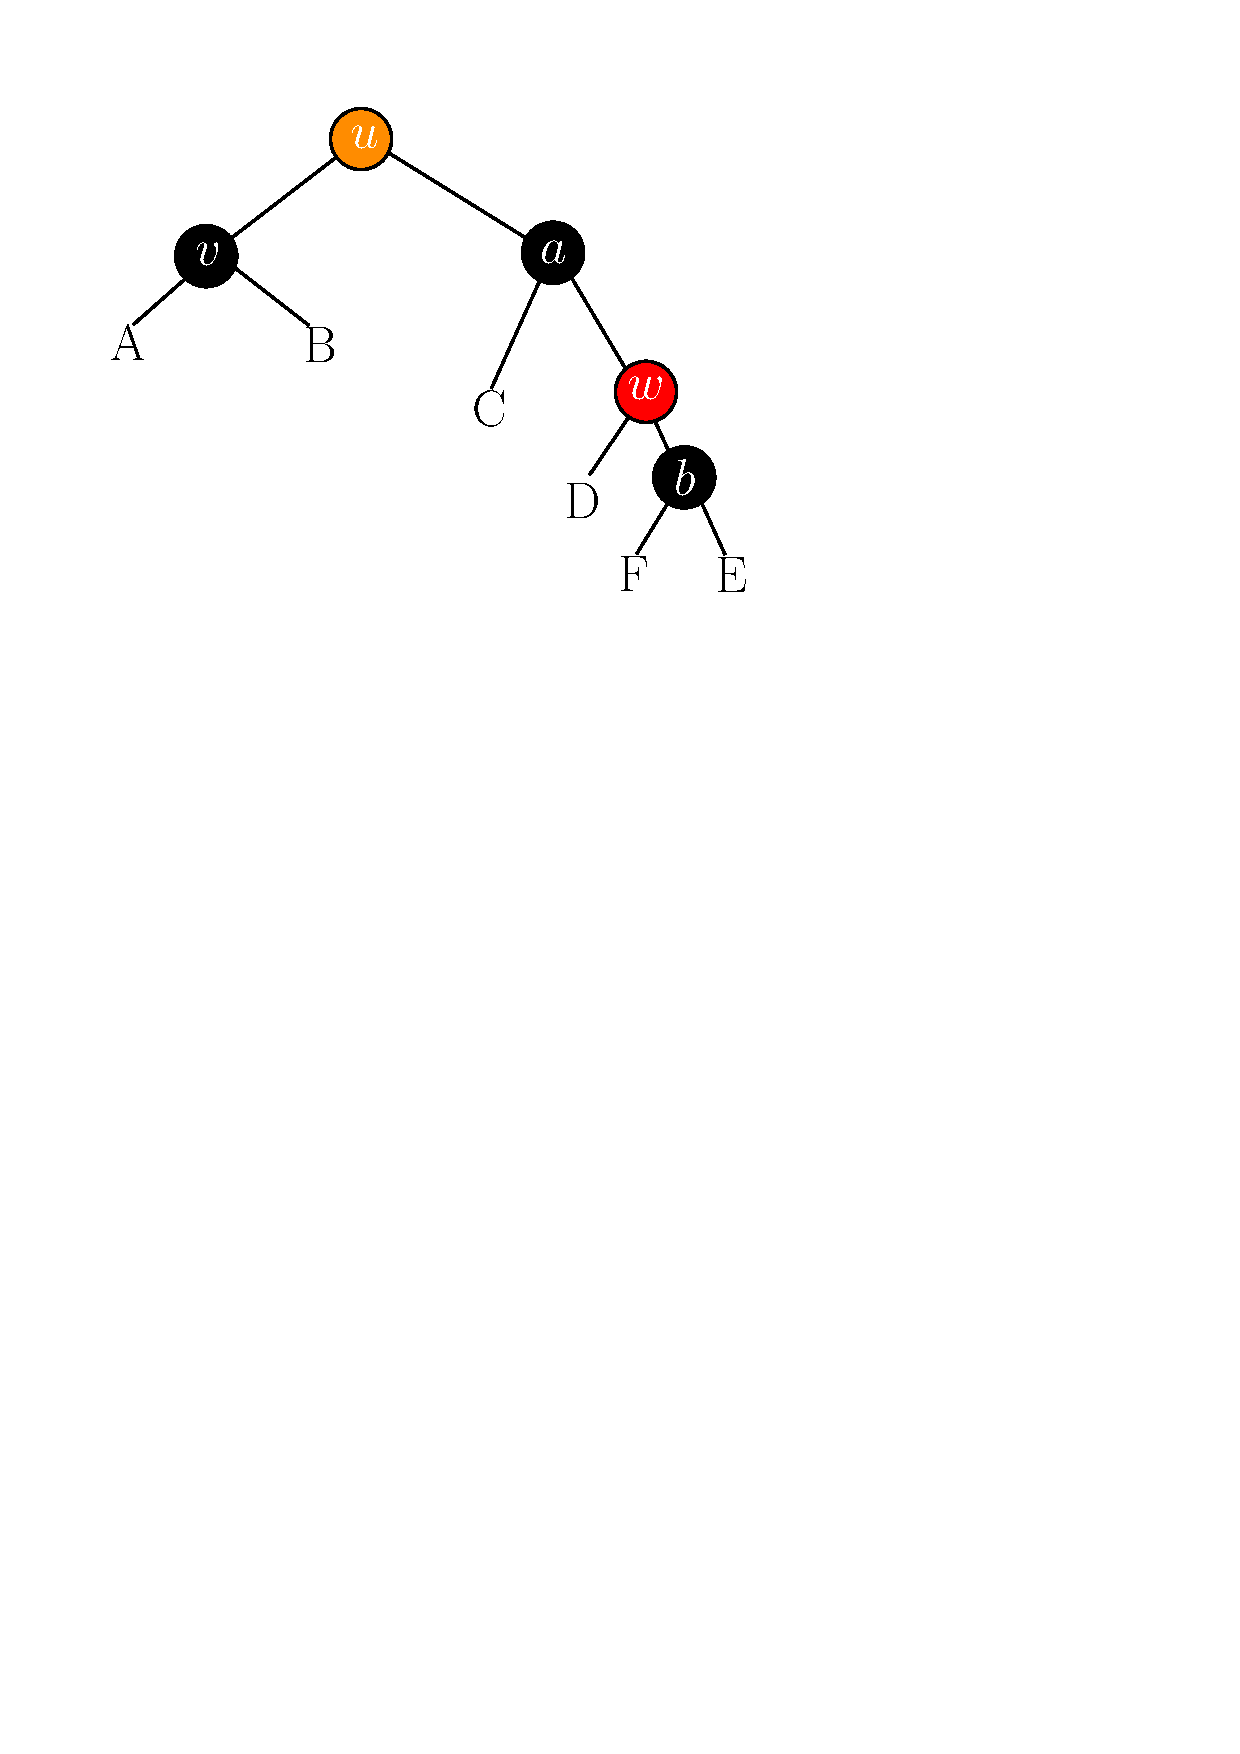
\includegraphics[height=30mm]{./images/rbtree_del_3a.pdf}
	\begin{exampleblock}{Fall 3: schwarzer Schwesterknoten $w$, linkes Kind von $w$ rot, rechtes Kind schwarz}
		\begin{itemize}
			\item vertausche die Farben von $w$ und seinem linken Kind
			\item Rechtsrotation um $w$
			\item fahre fort mit Fall 4, mit neuem Schwesterknoten $w=a$
		\end{itemize}
	\end{exampleblock}
\end{frame}

\begin{frame}\frametitle{\mytitle}
	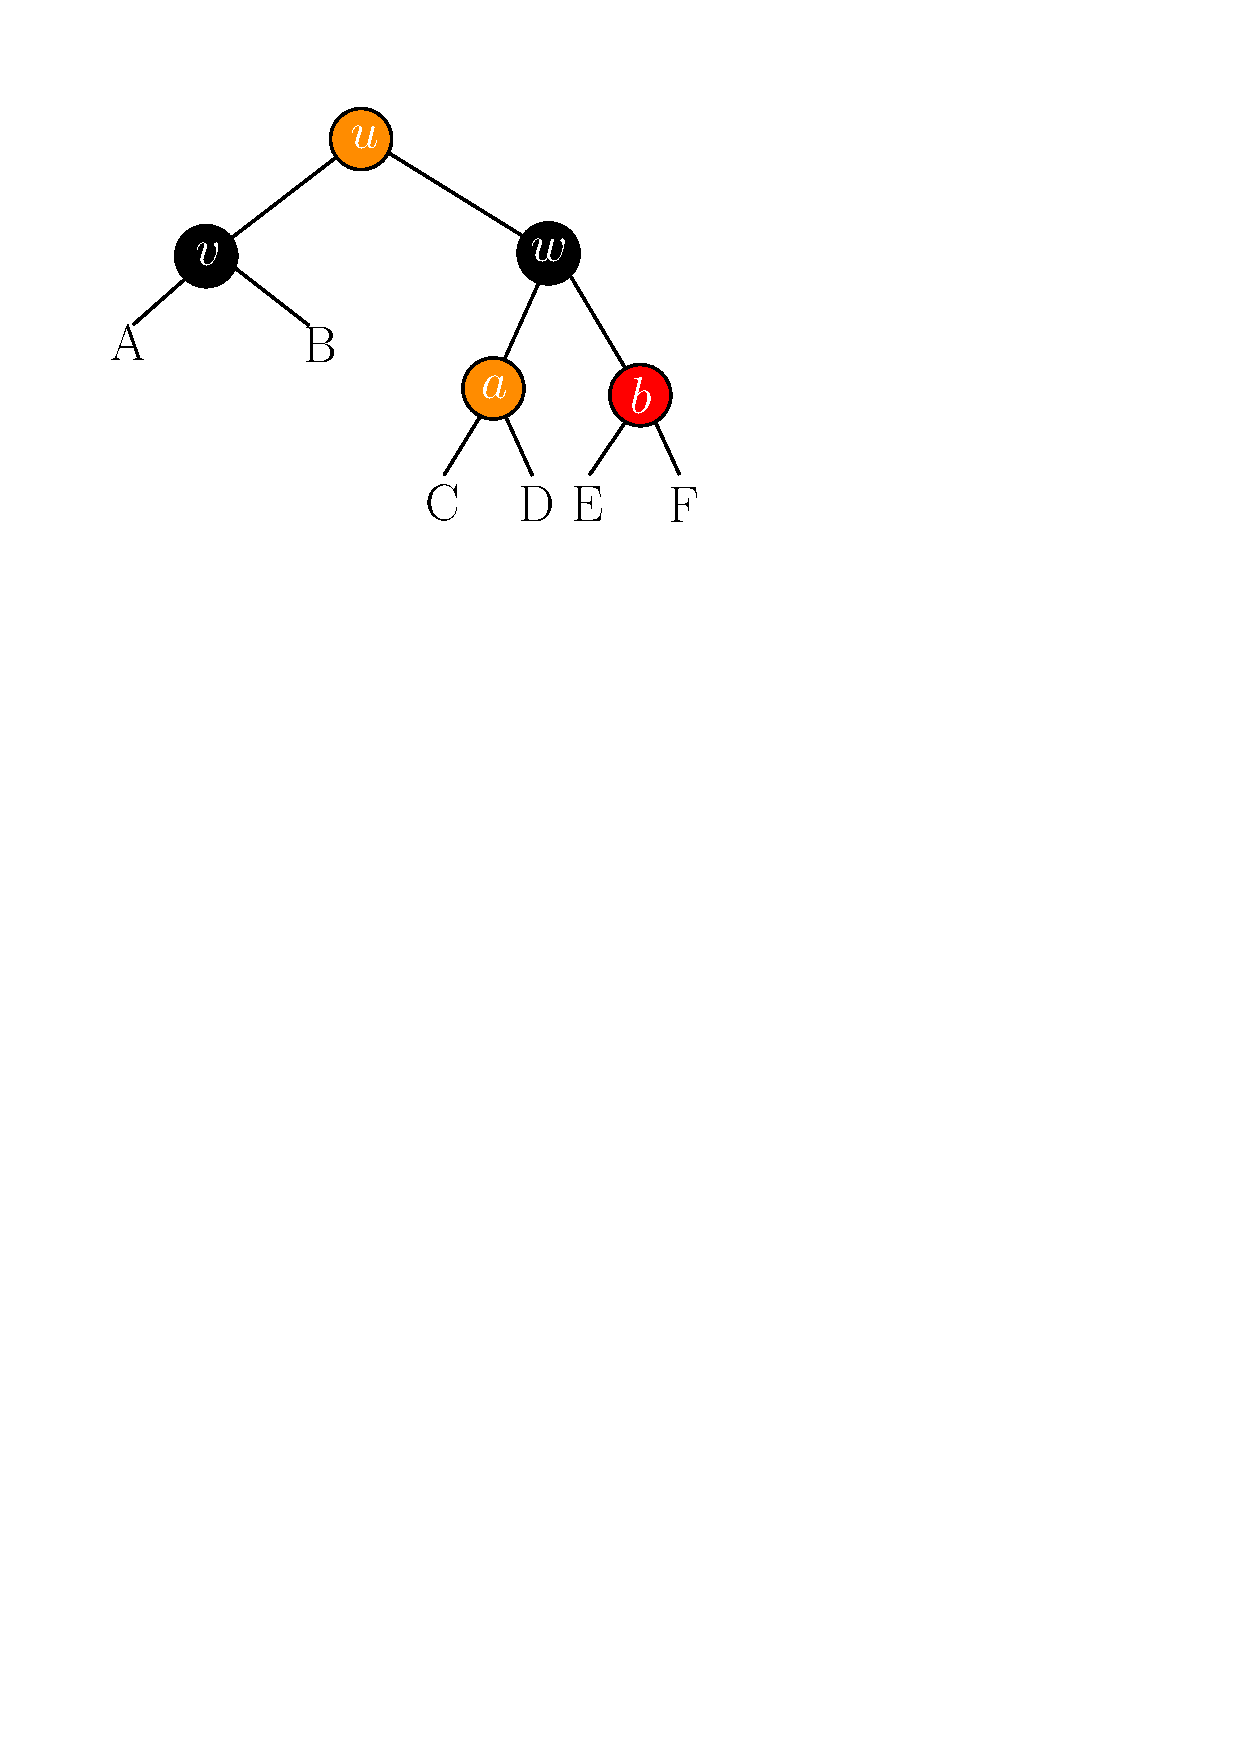
\includegraphics[height=30mm]{./images/rbtree_del_4.pdf}\hfill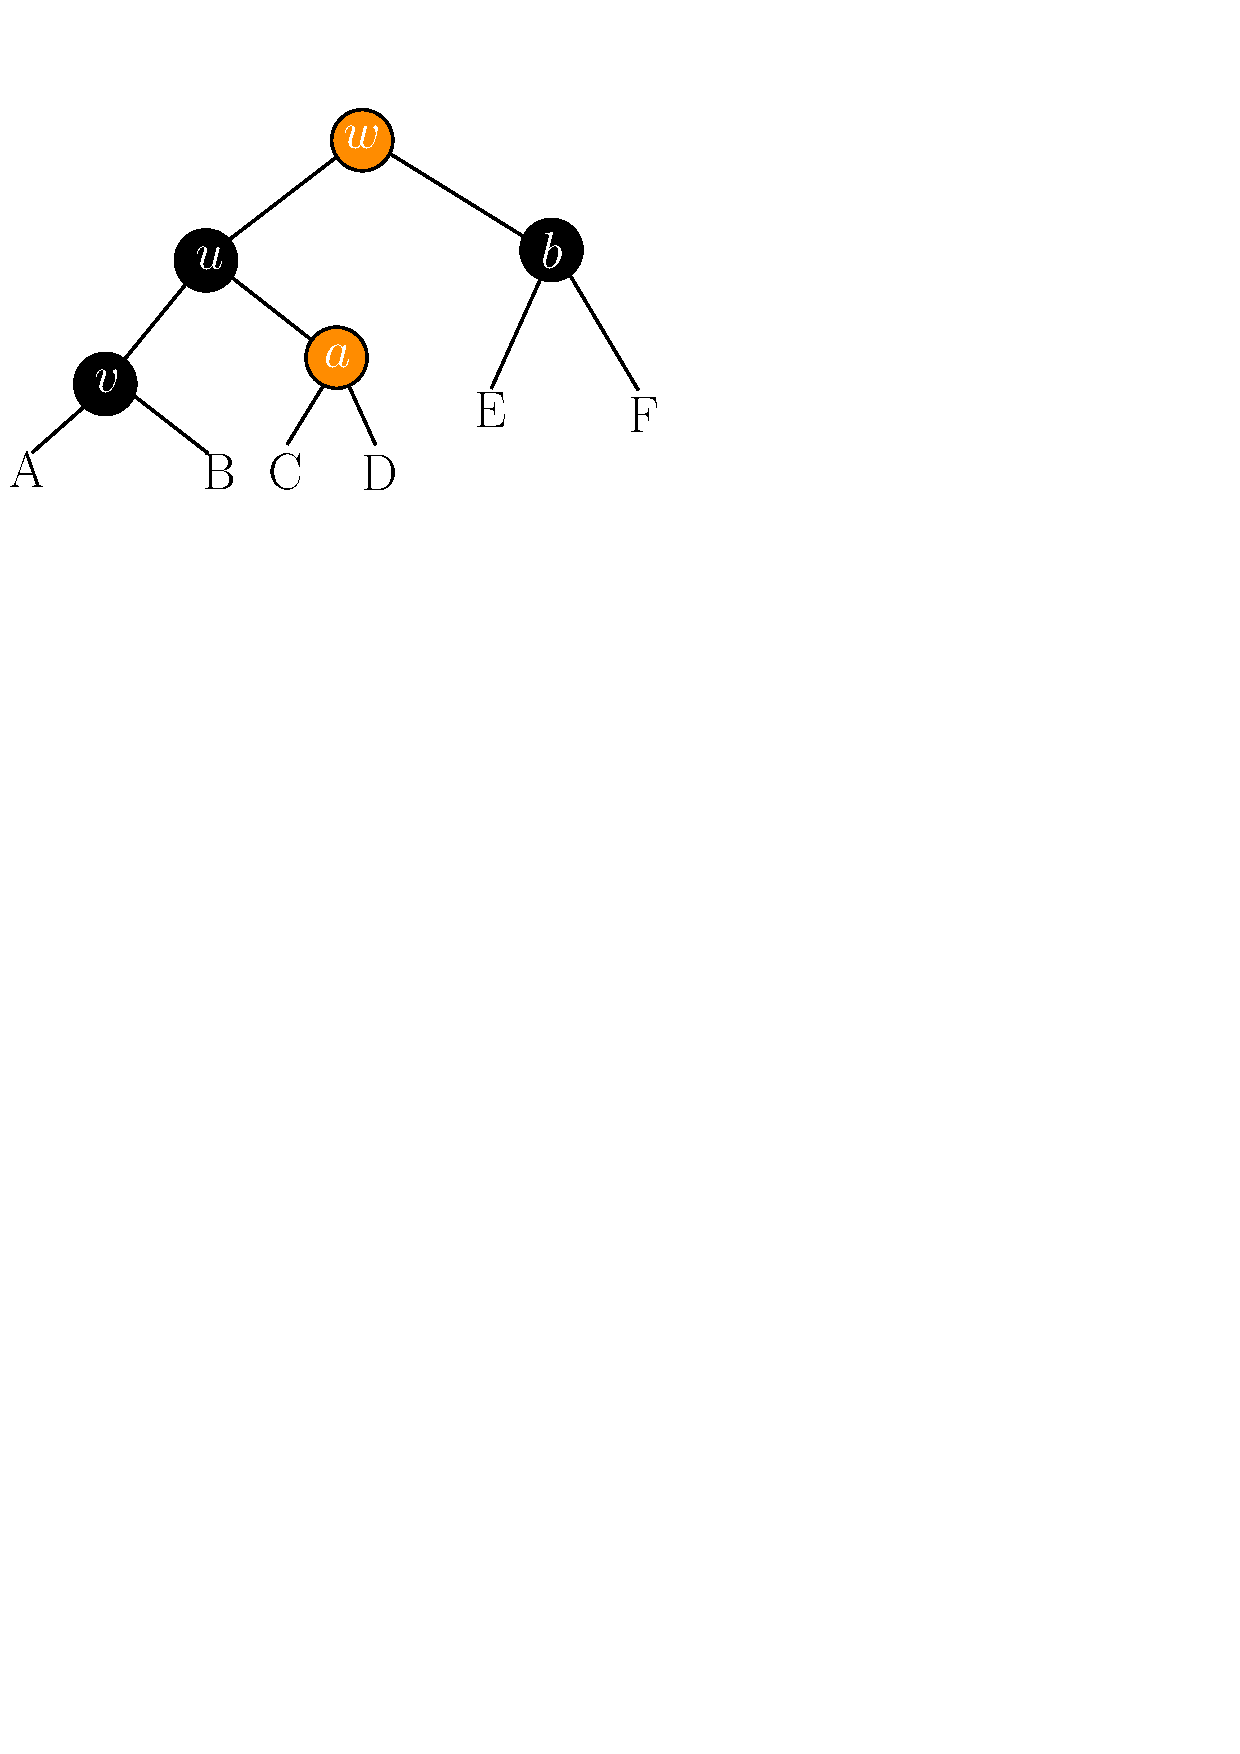
\includegraphics[height=30mm]{./images/rbtree_del_4a.pdf}
	\begin{exampleblock}{Fall 4: schwarzer Schwesterknoten $w$, rechtes Kind von $w$ rot}
		\begin{itemize}
			\item Linksrotation um $u$
			\item Farben anpassen $\leadsto$ Bedingung RB5 nun erf\"ullt; setze $v$ auf die Wurzel des Baums
		\end{itemize}
	\end{exampleblock}
\end{frame}

\begin{frame}\frametitle{\mytitle}
	\begin{exampleblock}{Abschlu\ss}
		\begin{itemize}
			\item sobald der aktuelle Knoten $v$ schwarz gef\"arbt ist, sind wir fertig
			\item wenn $v$ die Wurzel ist, f\"arben wir $v$ schwarz und sind dann ebenfalls fertig
		\end{itemize}
	\end{exampleblock}
\end{frame}

\begin{frame}\frametitle{\mytitle}
	\begin{block}{Proposition}
		Die Laufzeit zum Entfernen eines Knotens ist $O(\log n)$.
	\end{block}
	\begin{exampleblock}{Beweis}
		\begin{itemize}
			\item in den F\"allen 1,3 und 4 h\"alt der Algorithmus nach $O(1)$ Schritten
			\item in Fall 2 bewegen wir uns auf die Wurzel zu
		\end{itemize}
	\end{exampleblock}
\end{frame}

\begin{frame}\frametitle{\mytitle}
	\begin{exampleblock}{Zusammenfassung}
		\begin{itemize}
			\item red black trees sind extrem effiziente selbstbalancierende bin\"are Suchb\"aume
			\item \alert{Beispielanwendung:} Prozessorscheduling im Linux-Kern
		\end{itemize}
	\end{exampleblock}
\end{frame}

\end{document}
